\documentclass[a4paper, 12pt]{article}%тип документа

%отступы
\usepackage[left=2cm,right=2cm,top=2cm,bottom=3cm,bindingoffset=0cm]{geometry}

%Русский язык
\usepackage[T2A]{fontenc} %кодировка
\usepackage[utf8]{inputenc} %кодировка исходного кода
\usepackage[english,russian]{babel} %локализация и переносы

%Вставка картинок
\usepackage{wrapfig}
\usepackage{graphicx}
\graphicspath{{pictures/}}
\DeclareGraphicsExtensions{.pdf,.png,.jpg}

%оглавление
\usepackage{titlesec}
\titlespacing{\chapter}{0pt}{-30pt}{12pt}
\titlespacing{\section}{\parindent}{5mm}{5mm}
\titlespacing{\subsection}{\parindent}{5mm}{5mm}
\usepackage{setspace}

%Графики
\usepackage{multirow}
\usepackage{pgfplots}
\pgfplotsset{compat=1.9}

%Математика
\usepackage{amsmath, amsfonts, amssymb, amsthm, mathtools}

%Заголовок
\usepackage{lastpage} 
\usepackage{fancybox,fancyhdr}
\fancyhead[R]{\textit{Закон Кюри-Вейсса и обменное взаимодействие в ферромагнетиках}}
\fancyhead[L]{\textit{Работа 9.1 - 9.2}}
\fancyhead[C]{}

\newtheorem{task}{Задача}
\begin{document} 
		\begin{titlepage}
			\begin{center}
				\textit{Федеральное государственное автономное образовательное\\ учреждение высшего образования }
				\vspace{0.5ex}
				
				\textbf{«Московский физико-технический институт\\ (национальный исследовательский университет)»}
			\end{center}
			\vspace{10ex}
			\begin{center}
				\vspace{13ex}
				\textbf{Лабораторная работа №9.1}
				\vspace{1ex}
				
				по курсу основы современной физики
				
				
				на тему:
				
				\textbf{\large{<<Закон Кюри-Вейсса и обменное взаимодействие в ферромагнетиках>>}}
				
				\vspace{30ex}
				\begin{flushright}
					\noindent
					\textit{Работу выполнил:}
					\\
					\textit{Шелестов Федор
					}						 
				\end{flushright}
				\vfill
				Долгопрудный \\2021 год
			\end{center}
		\end{titlepage}
	
				\newpage
		
	
	\pagestyle{fancy}
	

\textbf{Цель работы:} исследовать температурную зависимость магнитной восприимчивости ферромагнетика в парамагнитной области -- выше точки Кюри. По полученной в работе температуре Кюри оценить энергия обменного взаимодействия. Объектом исследования является металлический гадолиний.

\section{Теоретическая справка}
\subsection{Феноменологическое описание ферромагнетиков: парамагнитная фаза и эффективное поле Вейсса}
Вещества, атомы которых обладают некомпенсированным магнитным моментом, принадлежат к парамагнетикам. В отсутствие внешнего магнитного поля магнитные моменты как атомов, так и свободных электронов направлены в разные стороны, так что суммарный магнитный момент вещества равен нулю. Во внешнем поле состояние, соответствующее направлению «по полю», оказываются энергетически более выгодными, и вещество намагничивается.
Намагниченностью называется магнитный момент $І$ единицы объёма, который связан с внешним магнитным полем $H$, под действием которого он возникает, соотношением:
$$
I = \varkappa H
$$
Константа $\chi$ называется магнитной восприимчивостью вещества. В вакууме в системе единиц Гаусса между напряжённостью поля $Н$ и индукцией поля В разницы нет.
Рассмотрим восприимчивость парамагнитного вещества, в котором магнитный момент атома обусловлен только спином одного электрона. Как известно, проекция спина на любое выделенное направление (в нашем случае - направиление магнитного поля) может быть равна либо $\hbar/2$ либо $-\hbar/2$. Проекция спинового магнитного момента электрона также может иметь соответственно два значения: $\mu_{z}= \pm \mu,$ где $\mu$ -- абсолютное значение проекции магнитного момента.
Взаимодействие магнитного момента $\vec{\mu}$ с внешним полем $\vec{B}$ приводит к дополнительной энергии $E=-\left(\vec{\mu} \cdot \vec{B}\right),$ зависящей от взаимной ориентации этих векторов. Следовательно в нашем случае в магнитном поле у атома возникают два возможных уровня энергии:
$$
E_{-}=-\mu B \quad \text { и } \quad E_{+}=+\mu B
$$

Причем в низкоэнергетичном состоянии $Е_-$ магнитный момент параллелен магнитному
полю.

В соответствии с Больцмановским распределением отношение числа электронов $N_{+}$ с 
энергией $E_{+}$ к числу электронов $N_-$ с энергией $E_-$ равно
$$
\frac{N_{+}}{N_{-}}=\exp \left(-\frac{2 \mu B}{k_{\mathrm{B}} T}\right) \simeq 1-\frac{2 \mu B}{k_{\mathrm{B}} T}
$$
Возможность замены экспоненты её приближенным выражением связана с тем, что
практически во всех магнитных полях магнитная энергия атомов много меньше
тепловой.

Намагниченность вещества определяется только разностью чисел электронов,
магнитные моменты которых ориентированы по полю или против поля.
$$
I=\mu \Delta N=N \frac{\mu^{2}}{k_{\mathrm{B}} T} H
$$
Парамагнитная часть восприимчивости равна:
$$\alpha = \frac{I}{H} = N \frac{\mu^2}{k_B T} = N \frac{\mu_B^2}{k_B T}$$
Данную формулу можно обобщить. Магнитный момент электрона $\mu$ связан с его
механическим моментом $Ј$ выражением
$$
\mu=g \mu_{\mathrm{B}} J
$$
Где $g$ -- фактор Ланде. 
В случае, если у атома более одного электрона, и суммарный спин атома равен $S$, то
$$
\left\langle\mathrm{S}^{2}\right\rangle=S(S+1)
$$
И квадрат магнитного момента равен
$$
\vec{\mu}^{2}=\mu^{2}=g^{2} \mu_{\mathrm{B}}^{2} S(S+1)
$$
В сферически симметричном состоянии выделенных осей нет, и поэтому
$$
\left\langle\mu^{2}\right\rangle=\left\langle\mu_{x}^{2}\right\rangle+\left\langle\mu_{y}^{2}\right\rangle+\left\langle\mu_{z}^{2}\right\rangle=3\left\langle\mu_{z}^{2}\right\rangle
$$

Таким образом, среднее значение квадрата проекции магнитного момента на любую
ось $z$ равно
$$
\left\langle\mu_{z}^{2}\right\rangle=\frac{1}{3} \mu^{2}=\frac{g^{2} \mu_{\mathrm{B}}^{2} S(S+1)}{3}
$$
Подставляя это выражение в первоначальную формулу магнитной восприимчивости, получим общее выражение
$$
\alpha=\frac{N g^{2} \mu_{\mathrm{B}}^{2} S(S+1)}{3 k_{\mathrm{B}} T}
$$
Полученная формула носит название Закона Кюри и показывает, что магнитная
восприимчивость парамагнетиков обратно пропорциональна температуре.
Рассмотрим теперь ферромагнетики. Феноменологическая теория ферромагнетизма
была построена П. Вейссом задолго до создания квантовой механики. Для описания
взаимодействия соседний электронов он предположил, что в ферромагнетике
имеется некоторое эффективное магнитное поле $H_{\text {эфф }}$ (это поле также называют обменным в силу его квантово-механической природы). Величина обменного поля пропорциональна имеющейся намагниченности образца (количеству электронов с
коррелированными направлениями магнитных моментов):

$$
H_{\text{эфф}} = \lambda I
$$

Где $\lambda$ -- некоторая константа, положительная у ферромагнетиков и отрицательная у антиферромагнетиков.

Выше температуры Кюри $T_c$ ферромагнетик является парамагнетиком -- тепловое
движение полностью разупорядочивает магнитные моменты атомов. Чтобыо писать зависимость восприимчивости ферромагнетика в парамагнитной области надо рассмотреть закон Кюри, учитывая поправку на дополнительное поле $H_{\text {эфф }}$
$$
I=N \frac{\mu^{2} H}{k_{\mathrm{B}}(T-\Theta)} 
$$
$$
\Theta=\frac{N \mu^{2} \lambda}{k_{\mathrm{B}}}=N \frac{g^{2} \mu_{\mathrm{B}}^{2} S(S+1)}{3 k_{\mathrm{B}}} \lambda
$$
$\Theta$ -- параметр, имеющий размерность температуры.
$$
\varkappa=\frac{I}{H}=N \frac{g^{2} \mu_{\mathrm{B}}^{2} S(S+1)}{3 k_{\mathrm{B}}(T-\Theta)} \propto \frac{1}{T-\Theta}
$$

Модифицированная формула Кюри носит название закон Кюри-Вейсса. Этот законносит приближенный характер и не позволяет описать, что происходит в ферромагнитой области, но температурную зависимость магнитной восприимчивости в парамагнитной фазе описывает неплохо. 
\subsection{Связь эффективного поля Вейсса с обменным интегралом.}
В теории Гейзенберга-Френкеля энергия $U_\text{обм}$ обменного взаимодейтвия атомов $i$ и $j$ выражается соотношением
$$
U_\text{обм} = -2 J S_i S_j
$$
Энергия $U$ представляет собой разность между средними значениями кулоновской энергии для параллельных и антипараллельных спинов $S_i$ и $S_j$, а $Ј$ -- коэффициент пропорциональности, называемый обменным интегралом, величина которого зависит от
степени перекрытия распределённых зарядов атомов $i$ и $ј$ (от степени перекрытия
волновых функций электронов).

Установим приближенно связь между обменным интегралом $Ј$ и константой Вейсса $\lambda$. Предположим, что рассматриваемый атом имеет $n$ ближайших соседей, и обменное
взаимодействие каждого из них с центральным атомом одинаково, а для более далеких соседей будем считать обменный интеграл равным нулю, так как обменное взаимодействие быстро убывает с ростом расстояния между атомами. Найдем энергию $U_\text{пер}$, требуемую
для переворота данного спина в присутствии всех других спинов. Эта энергия вдвое больше обменной энергии системы с какой-то определенной ориентацией спина, так как $\mathrm{U}_{\uparrow \uparrow}=-\mathrm{U}_{\uparrow \downarrow}$ поэтому её можно записать в следующем виде:
$$
U_{\text {пер }} \simeq 2\left(2 J n S^{2}\right)
$$
При феноменологическом описании каждый магнитный атом испытывает действие
эффективного поля, пропорционального намагниченности, а намагниченность по
определению есть магнитный момент единицы объёма. Иначе говоря, воздействиевсех спинов на данный характеризуется средней намагниченностью $І=\mu/V$, и мы можем
записать энергию переворота в виде
$$
U_{\mathrm{rrep}}=2 \mu H_{\text {эфф }}=2 \mu(\lambda I)=2 \mu \frac{\lambda \mu}{V}
$$

Где $V$ -- объём, приходящийся на один атом. Средний магнитный момент электрона, обусловленный его спином, есть $\mu=g S \mu_{\text{B}}$. Следовательно, для константы Вейсса $\lambda$ мы получаем следующее выражение:

$$
\lambda=\frac{2 n J V}{g^{2} \mu_{\mathrm{B}}^{2}}
$$

Так как объём, занимаемый одним атомом, равен $V=1/N$, где $N$ -- концентрация атомов, то мы окончательно получаем:

$$
J=\frac{3 k_{\text {B }} \Theta}{2 n S(S+1)}
$$
\newpage
\section{Экспериментальная установка и принцип измерений}

\begin{figure}[h!]
\begin{center}
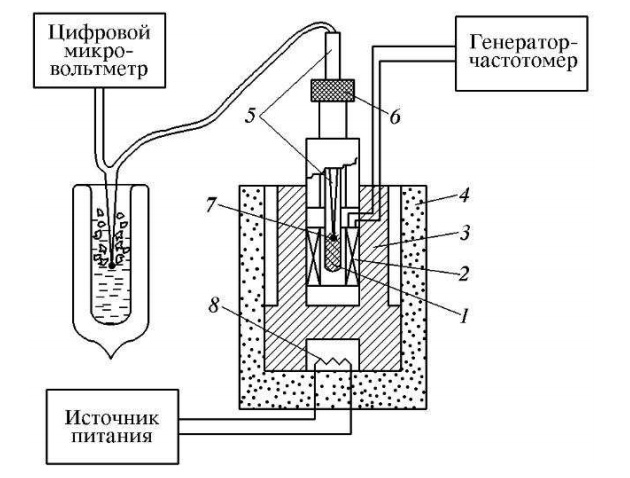
\includegraphics[scale=0.7]{1.jpg}
\caption{Схема экспериментальной установки: 1 -- капсула с образцом; 2-- катушка самоиндукции; 3 -- медный цилиндр; 4 -- пенопластовый корпус; 5 -- шток; 6 -- цанговый зажим; 7 -- измерительный спай термопары; 8 -- электронагреватель}
\end{center}
\end{figure}

Экспериментальная установка для измерения восприимчивости магнетиков приведена на рис. 1.  Ферромагнитный образец 1 располагается внутри пустотелой катушки 2, которая является индуктивностью колебательного контура, входящего в состав LC-генератора. Генератор собран на полевом транзисторе и смонтирован в виде отдельного блока. Частота колебаний генератора высвечивается на цифровом табло блока. Катушка самоиндукции помещена в термостат, представляющий собой массивный медный цилиндр 3, расположенный в пенопластовом корпусе 4. Исследуемый ферромагнетик (гадолиний) является проводником электрического тока, а рабочая частота генератора довольно высока -- порядка сотен килогерц. Поэтому для того, чтобы в образце не возникали токи Фуко, маскирующие изучаемый эффект, он изготовлен из мелких гранул размером менее 0,1 мм. Образец помещен в тефлоновую капсулу. С помощью штока 5 капсулу можно перемещать вдоль оси катушки самоиндукции. Когда шток опущен, образец введен в катушку, а когда поднят -- образец из неё вынут.

Магнитная восприимчивость образца определяется по изменению самоиндукции, происходящему при его введении в катушку. Обозначая через $L$ индуктивность катушки с образцом и через $L_0$ её индуктивность в отсутствии образца, получим:

$$
L=\mu \frac{4 \pi n^{2} S}{l} ; L_{0}=\frac{4 \pi n^{2} S}{l}
$$

Где $\mu$ -- магнитная проницаемость образца, $n$ -- число витков катушки, $l$ -- длина катушки, $S$ -- её сечение. Тогда

$$
\frac{L-L_{0}}{L_{0}}=\frac{\Delta L}{L_{0}}=\mu-1
$$
Так как длина образца существенно больше его диаметра, то размагничивающим
фактором можно пренебречь, и тогда получается, что:
$$
\frac{L-L_{0}}{L_{0}}=\mu-1=4 \pi \varkappa
$$
Учитывая, что частота $f$ колебательного LС-контура определяется выражением $\frac{1}{f}=2 \pi \sqrt{L C},$
получим:
$$
\frac{f_{0}^{2}-f^{2}}{f^{2}}=4 \pi \varkappa
$$
Отсюда следует, что
$$
\frac{1}{\varkappa} \propto \frac{f^{2}}{f_{0}^{2}-f^{2}}
$$
Измерения проводятся в интервале температур от $0^{\circ} \mathrm{ C}$ до $50^{\circ} \mathrm{ C} .$ Охлаждение образца производится с помощью массивного медного цилиндра 3, который предварительно охлаждается в морозильнике бытового холодильника или при помощи жидкого азота (77 К). Для нагревания служит электронагреватель 8, находящийся в тепловом контакте с
цилиндром 3. С целью экономии времени следует начинать измерения с малых
температур.

Температура образца измеряется медно-константановой термопарой, соединенной с цифровым микровольтметром. Чувствительность термопары 41 $\text{мкВ}/^\circ \text{С}$ . Один из спаев термопары находится в тепловом контакте с образцом, другой её спай термостатируется при 0 $  ^\circ \text{С}$ в сосуде Дьюара с тающим льдом. Источник питания нагревателя смонтирован в отдельном блоке. 

При выполнении работы образец сначала охлаждается ниже точки Кюри, а затем медленно нагревается. При этом исследуется зависимость частоты колебаний генератора от температуры образца. По зависимости $\frac{f^2}{f_0^2-f^2}$ от температуры проверяется справедливость закона Кюри-Вейсса и оценивается точка Кюри. Используя закон Кюри-Вейсса, определяют величину объемного интеграла исследуемого ферромагнетика. 
\newpage
\section{Измерения. Обработка результатов. Для Кюри-Вейса}
\begin{table}[h]
\begin{tabular}{|c|c|c|c|c|c|c|c|c|c|}
\hline
$U_{first}$, мВ & U, мв & T, C  & $\sigma_T$, C & T, K  & $\sigma_T$, K & $f_0$, кГц & f, кГц  & $\frac{f^2}{f_0^2-f^2}$ & $\sigma_{\frac{f^2}{f_0^2-f^2}}$ \\ \hline
-1,1            & 0,04  & 1     & 1,25          & 274,2 & 1,3           & 847        & 830,636 & 25,13                   & 0,04                             \\ \hline
-0,9            & 0,24  & 6,15  & 1,28125       & 279,3 & 1,3           & 846,2      & 830,9   & 26,91                   & 0,05                             \\ \hline
-0,8            & 0,34  & 8,7   & 1,279412      & 281,9 & 1,3           & 846,98     & 831,18  & 26,06                   & 0,05                             \\ \hline
-0,7            & 0,44  & 11,23 & 1,276136      & 284,4 & 1,3           & 847,03     & 831,65  & 26,79                   & 0,05                             \\ \hline
-0,6            & 0,54  & 13,77 & 1,275         & 286,9 & 1,3           & 847,75     & 832,5   & 27,05                   & 0,05                             \\ \hline
-0,5            & 0,64  & 16,28 & 1,271875      & 289,4 & 1,3           & 851,05     & 833,43  & 23,4                    & 0,04                             \\ \hline
-0,43           & 0,71  & 18    & 1,267606      & 291,2 & 1,3           & 847,96     & 836,71  & 36,94                   & 0,08                             \\ \hline
-0,35           & 0,79  & 20    & 1,265823      & 293,2 & 1,3           & 851,36     & 843,2   & 51,42                   & 0,12                             \\ \hline
-0,3            & 0,84  & 21,25 & 1,264881      & 294,4 & 1,3           & 853,6      & 846,7   & 61,1                    & 0,2                              \\ \hline
-0,2            & 0,94  & 23,73 & 1,262234      & 296,9 & 1,3           & 856,4      & 851     & 78,5                    & 0,2                              \\ \hline
-0,1            & 1,04  & 26,17 & 1,258173      & 299,3 & 1,3           & 857,8      & 853,5   & 99                      & 0,3                              \\ \hline
0,1             & 1,24  & 31    & 1,25          & 304,2 & 1,3           & 858,6      & 855,2   & 125,5                   & 0,5                              \\ \hline
0,2             & 1,34  & 33,48 & 1,249254      & 306,6 & 1,2           & 860        & 857,2   & 152,8                   & 0,6                              \\ \hline
0,3             & 1,44  & 35,88 & 1,245833      & 309   & 1,2           & 862,2      & 859,6   & 165,1                   & 0,7                              \\ \hline
0,4             & 1,54  & 38,29 & 1,243182      & 311,4 & 1,2           & 862,5      & 860     & 171,8                   & 0,7                              \\ \hline
0,47            & 1,61  & 40    & 1,242236      & 313,2 & 1,2           & 862,7      & 860,1   & 165,2                   & 0,7                              \\ \hline
0,6             & 1,74  & 43    & 1,235632      & 316,2 & 1,2           & 862,9      & 860,4   & 171,8                   & 0,7                              \\ \hline
0,7             & 1,84  & 45,4  & 1,233696      & 318,6 & 1,2           & 863,2      & 860,73  & 174                     & 0,8                              \\ \hline
0,8             & 1,94  & 47,76 & 1,230928      & 320,9 & 1,2           & 863,56     & 861,13  & 176,9                   & 0,8                              \\ \hline
\multicolumn{10}{|c|}{$\sigma_U = 0,05$ мВ, $\sigma_f = 0,2$ кГц}                                                                                           \\ \hline
\end{tabular}
\end{table}
По этим данным построим график (см. следующую страницу).

Температуру находим из градуировочной таблицы для медь-константановой термопары.
\begin{figure}[h]
\begin{center}
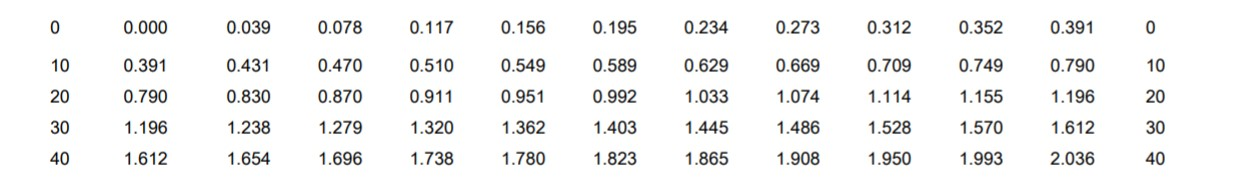
\includegraphics[width = \textwidth]{6.jpg}
\caption{Градуировка термопары}
\end{center}
\end{figure}

Несмотря на то, что параметр $\theta$ в законе Кюри-Вейсса больше температуры Кюри, пренебрежём этим расхождением, приравняем температуру Кюри гадолиния к $\theta$ и с помощью линеаризованной части графика и метода наименьших квадратов определим её.

Из теории парамагнитной области ферромагнетика и устройства экспериментальной установки мы знаем, что:

\[\frac{1}{\chi} \sim \frac{f^2}{f_0^2-f^2}\]
\[\frac{1}{\chi} \sim T - \theta\]
Отсюда следует, что 
\[\frac{f^2}{f_0^2-f^2} = \alpha \left( T - \theta \right)\]

где $\alpha$ - некоторая константа, которую мы можем найти с помощью метода наименьших квадратов для линеаризованной части. Таким образом, $\theta$ можно найти как точку пересечения прямой с осью ОХ. Погрешности также рассчитаем по закону наименьших квадратов.

\begin{figure}[h]
\begin{center}
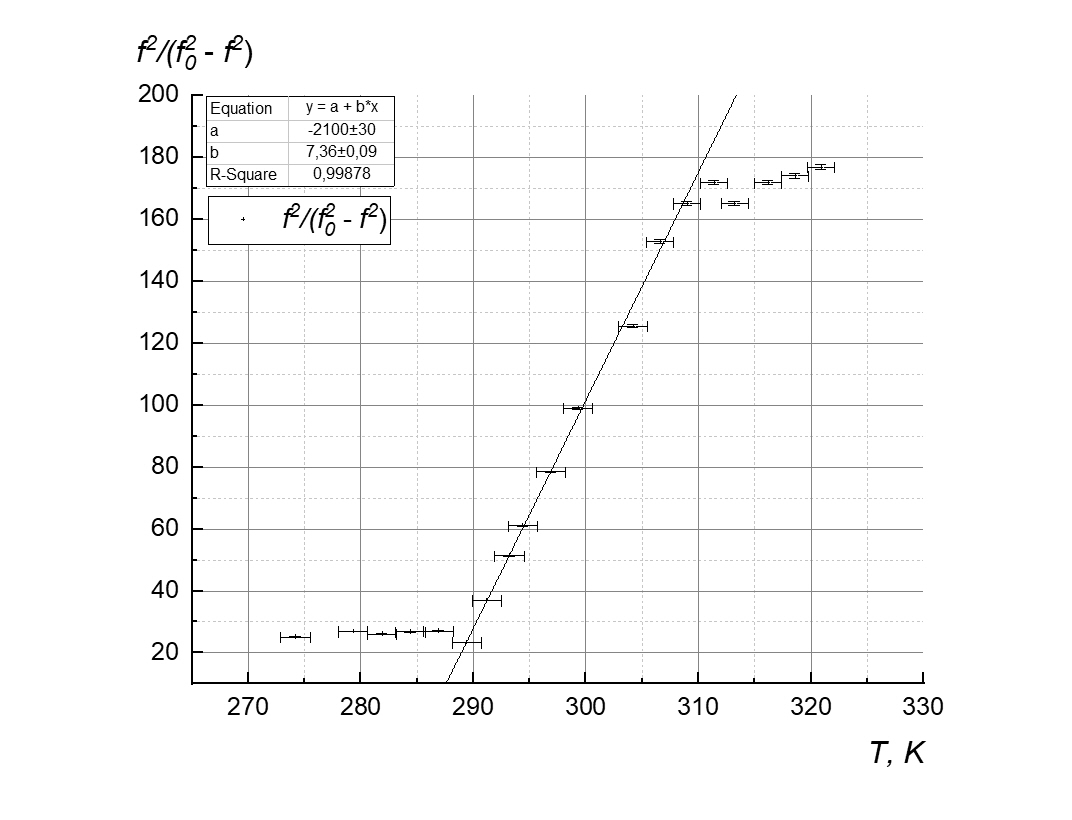
\includegraphics[width = \textwidth]{5.jpg}
\caption{Экспериментальная зависимость и линеаризация участка для определения параметра $\theta$}
\end{center}
\end{figure}

Из графика:
\[\alpha = (7,36 \pm 0,09) 1/K\]
\[\beta = -\alpha \theta = -2100 \pm 30\]

Тогда, мы можем найти параметр $\theta$:
\[\theta = -\frac{\beta}{\alpha} = (285 \pm 5) K\]
Где погрешность найдена по формуле, приведенной ниже:
\[\sigma_{\theta} = \theta \cdot \sqrt{\left(\frac{\sigma_{\alpha}}{\alpha}\right)^2 + \left(\frac{\sigma_{\beta}}{\beta}\right)^2}\]

Для того, чтобы оценить значение обменного интеграла воспользуемся формулой из теории:
\[J = \frac{3 k \theta}{2nS\left(S+1\right)}\]
\[\sigma_J = J \cdot \frac{\sigma_{\theta}}{\theta}\]
Для $n = 12$ и $S = 7/2$ получаем, что 
\[J = \left(2,91 \pm 0,05\right) K\]
\[J = \left(0,246 \pm 0,007\right) \text{мэВ}\]
\section{Измерения и анализ доменной структуры}
\begin{table}[h]
\begin{center}
\begin{tabular}{|c|c|c|c|c|c|c|c|c|}
\hline
$N$        & $I$, А        & $U$, В        & $\frac{I_0 - I}{I_0 + I}$ & $\sigma_{\frac{I_0 - I}{I_0 + I}}$ & $d$, пикс & $D$, пикс & $b$, мкм & $\sigma_b$, мкм \\ \hline
1          & 0             & 0             & 1                         & 0,06                               & 17        & 2142      & 79       & 5               \\ \hline
2          & 0,04          & 2             & 0,83                      & 0,05                               & 15        & 2121      & 71       & 5               \\ \hline
3          & 0,075         & 4             & 0,71                      & 0,05                               & 13        & 2129      & 61       & 5               \\ \hline
4          & 0,11          & 6             & 0,6                       & 0,04                               & 14        & 2040      & 69       & 5               \\ \hline
5          & 0,14          & 8             & 0,52                      & 0,04                               & 12        & 2052      & 58       & 5               \\ \hline
6          & 0,18          & 10            & 0,42                      & 0,04                               & 12        & 2054      & 58       & 5               \\ \hline
7          & 0,22          & 12            & 0,33                      & 0,03                               & 10        & 2053      & 49       & 5               \\ \hline
8          & 0,25          & 14            & 0,28                      & 0,03                               & 9         & 2134      & 42       & 5               \\ \hline
9          & 0,29          & 16            & 0,21                      & 0,03                               & 8         & 2167      & 37       & 5               \\ \hline
10         & 0,32          & 18            & 0,16                      & 0,03                               & 6         & 2089      & 29       & 5               \\ \hline
\multicolumn{3}{|c|}{$\sigma_I = 0,01$, A} & \multicolumn{3}{c|}{$I_0 = 0,44$ А}                                        & \multicolumn{3}{c|}{$U_0 = 24,6$ В}    \\ \hline
\end{tabular}

\end{center}
\end{table}

\begin{figure}[h]
\begin{center}
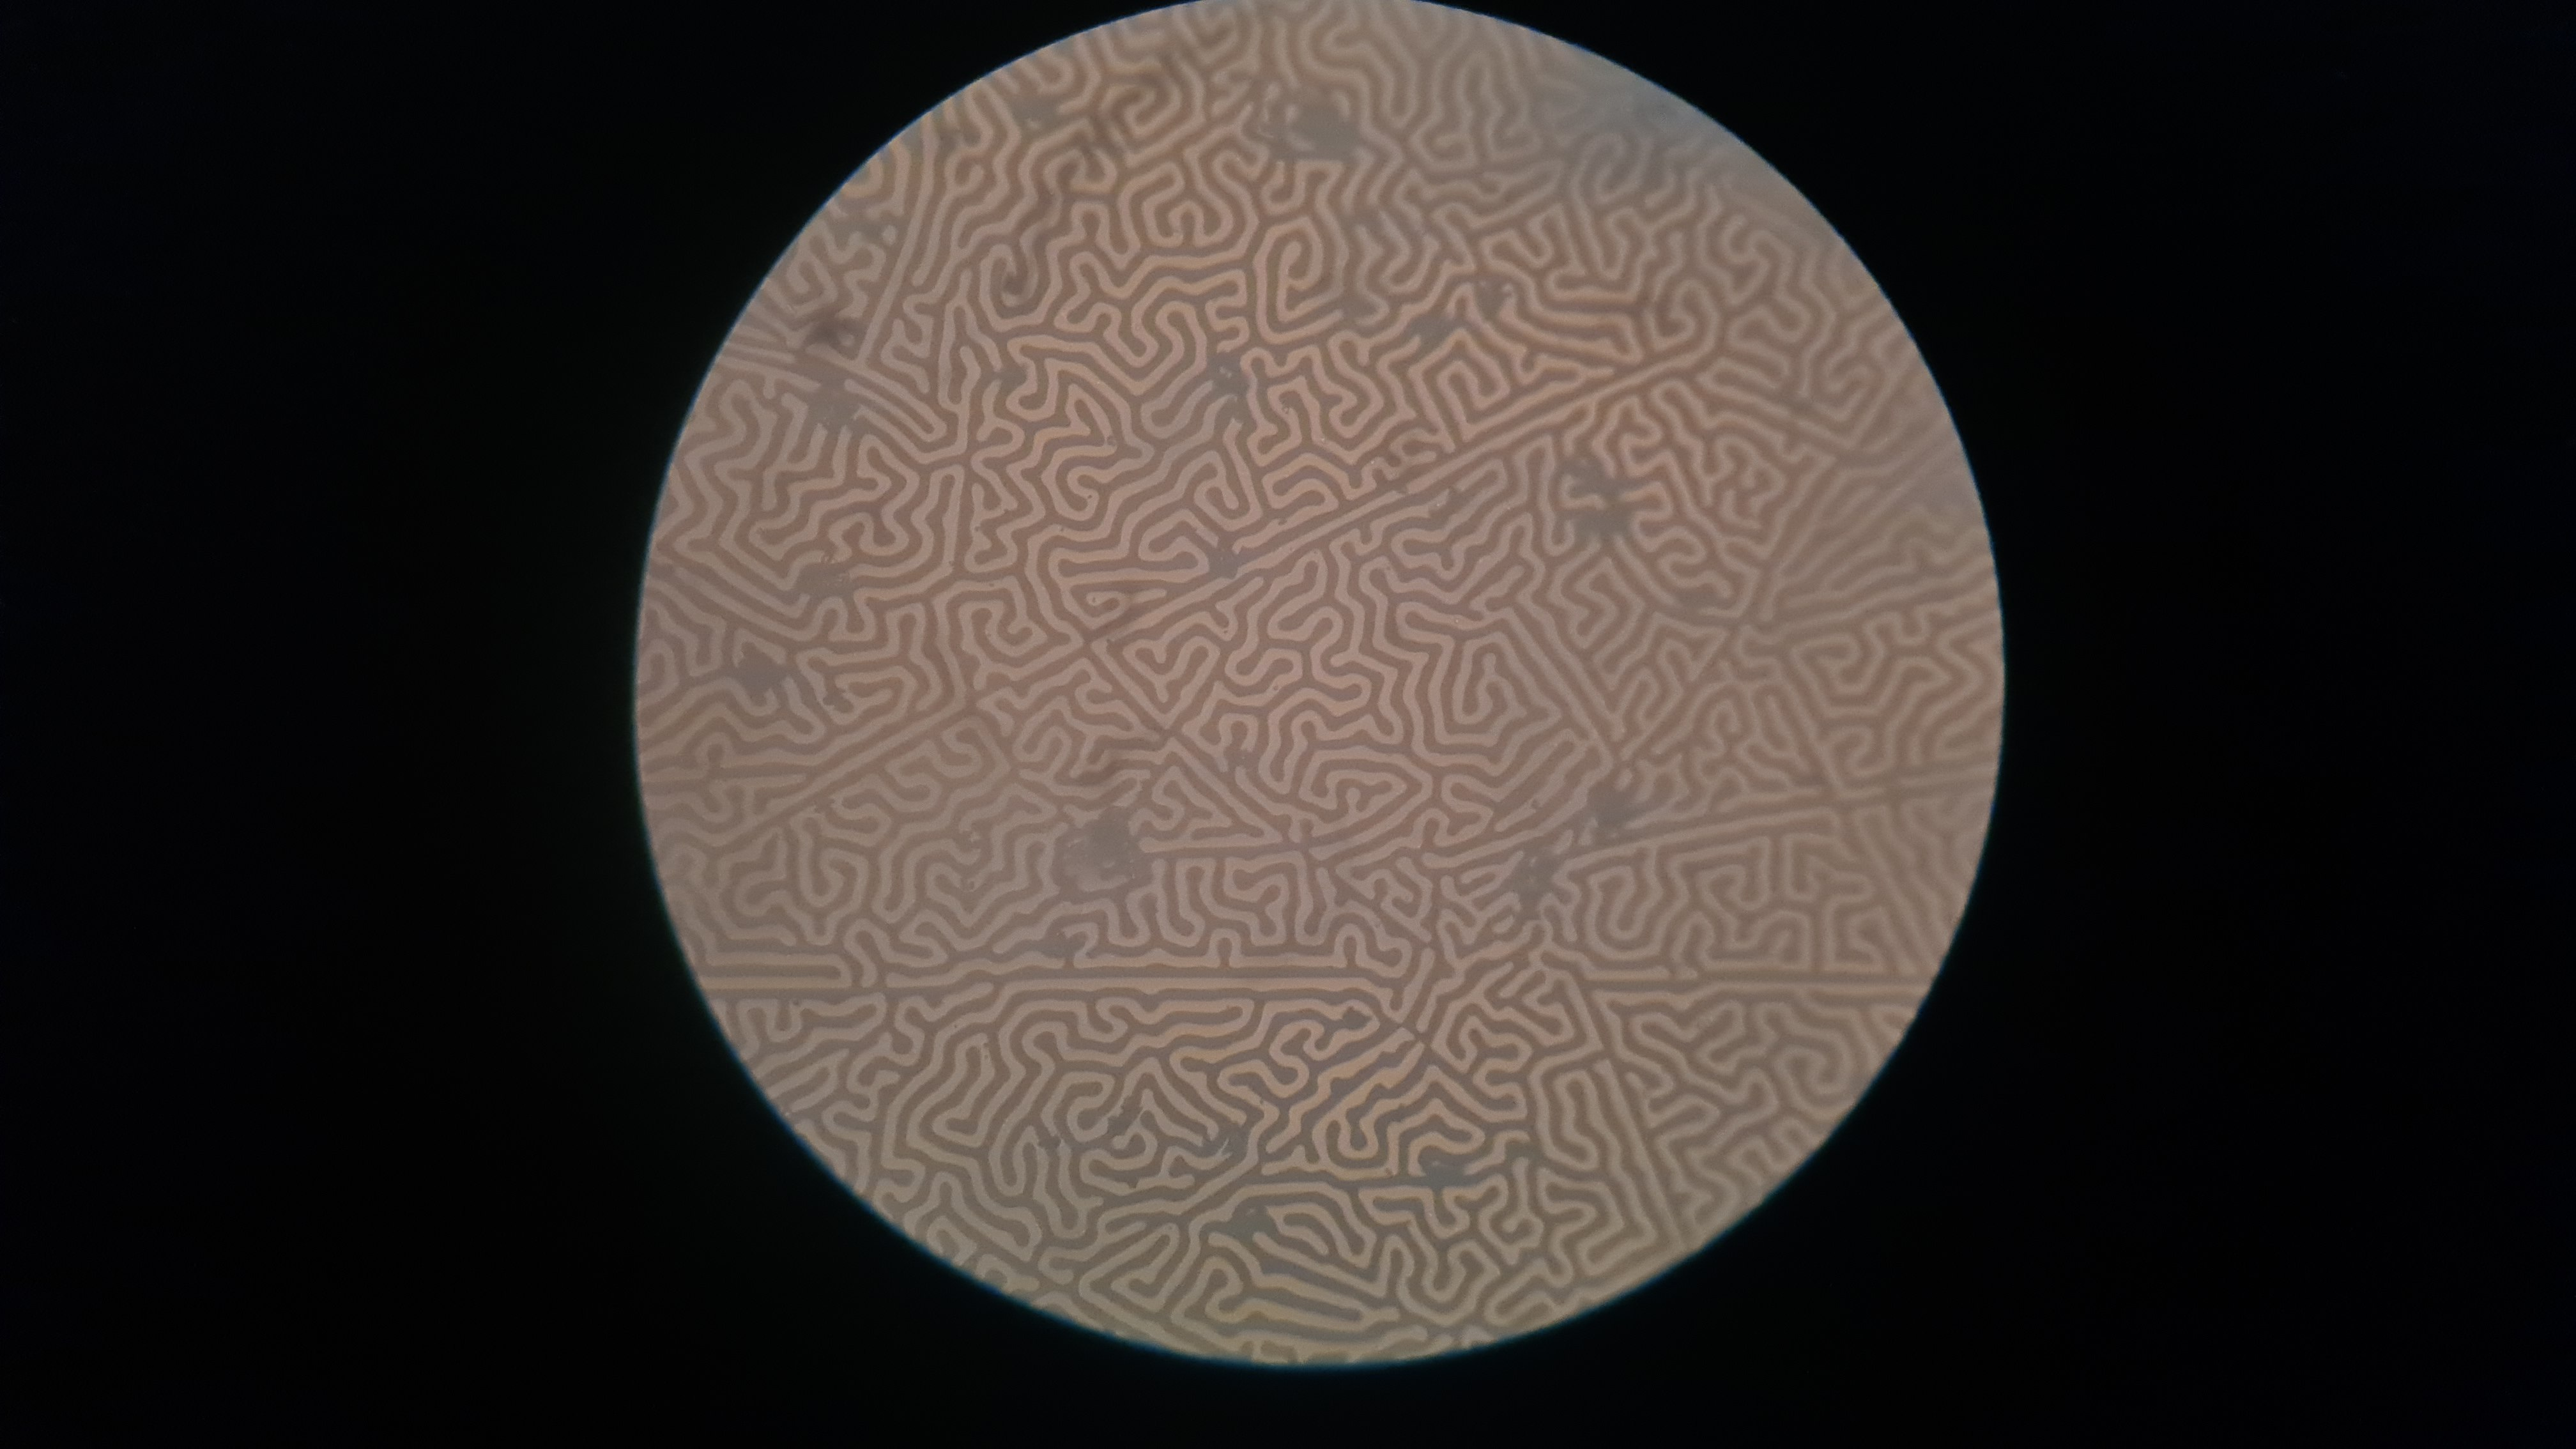
\includegraphics[width = 0.45\textwidth]{11.jpg}
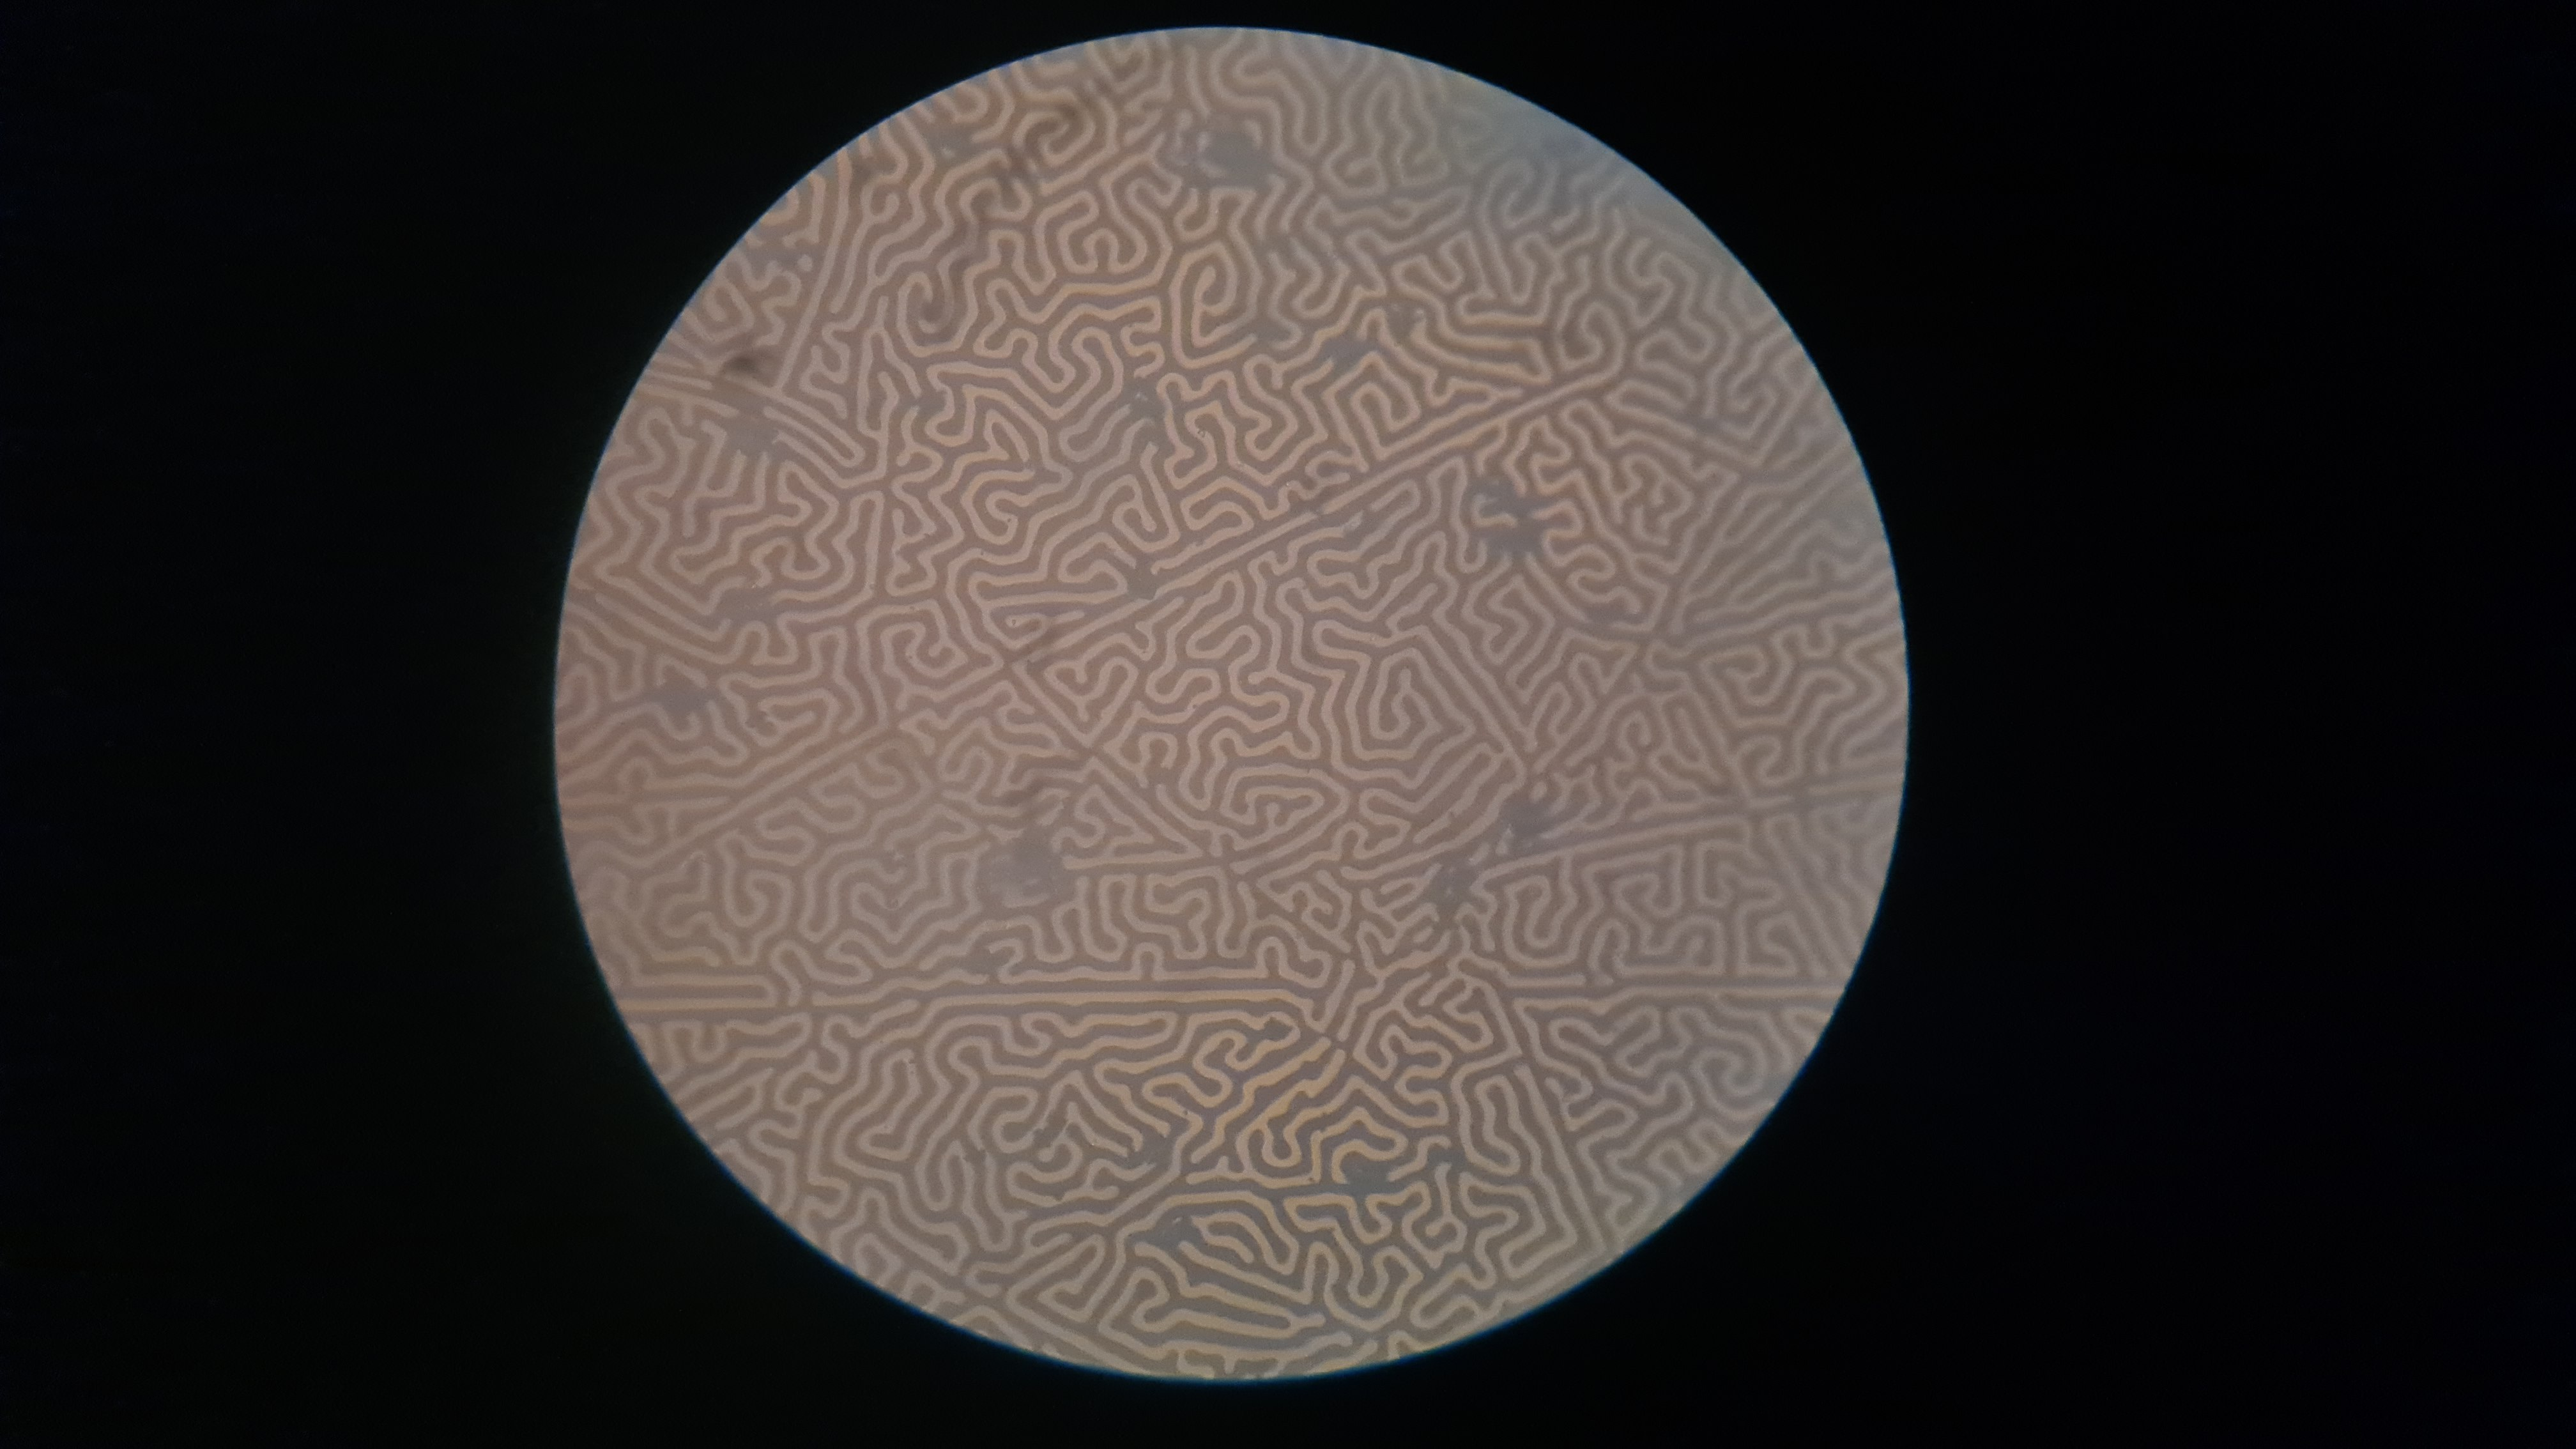
\includegraphics[width = 0.45\textwidth]{12.jpg}
\caption{Фото под номером 1 и 2 в таблице}
\end{center}
\end{figure}
\newpage
\begin{figure}[h]
\begin{center}
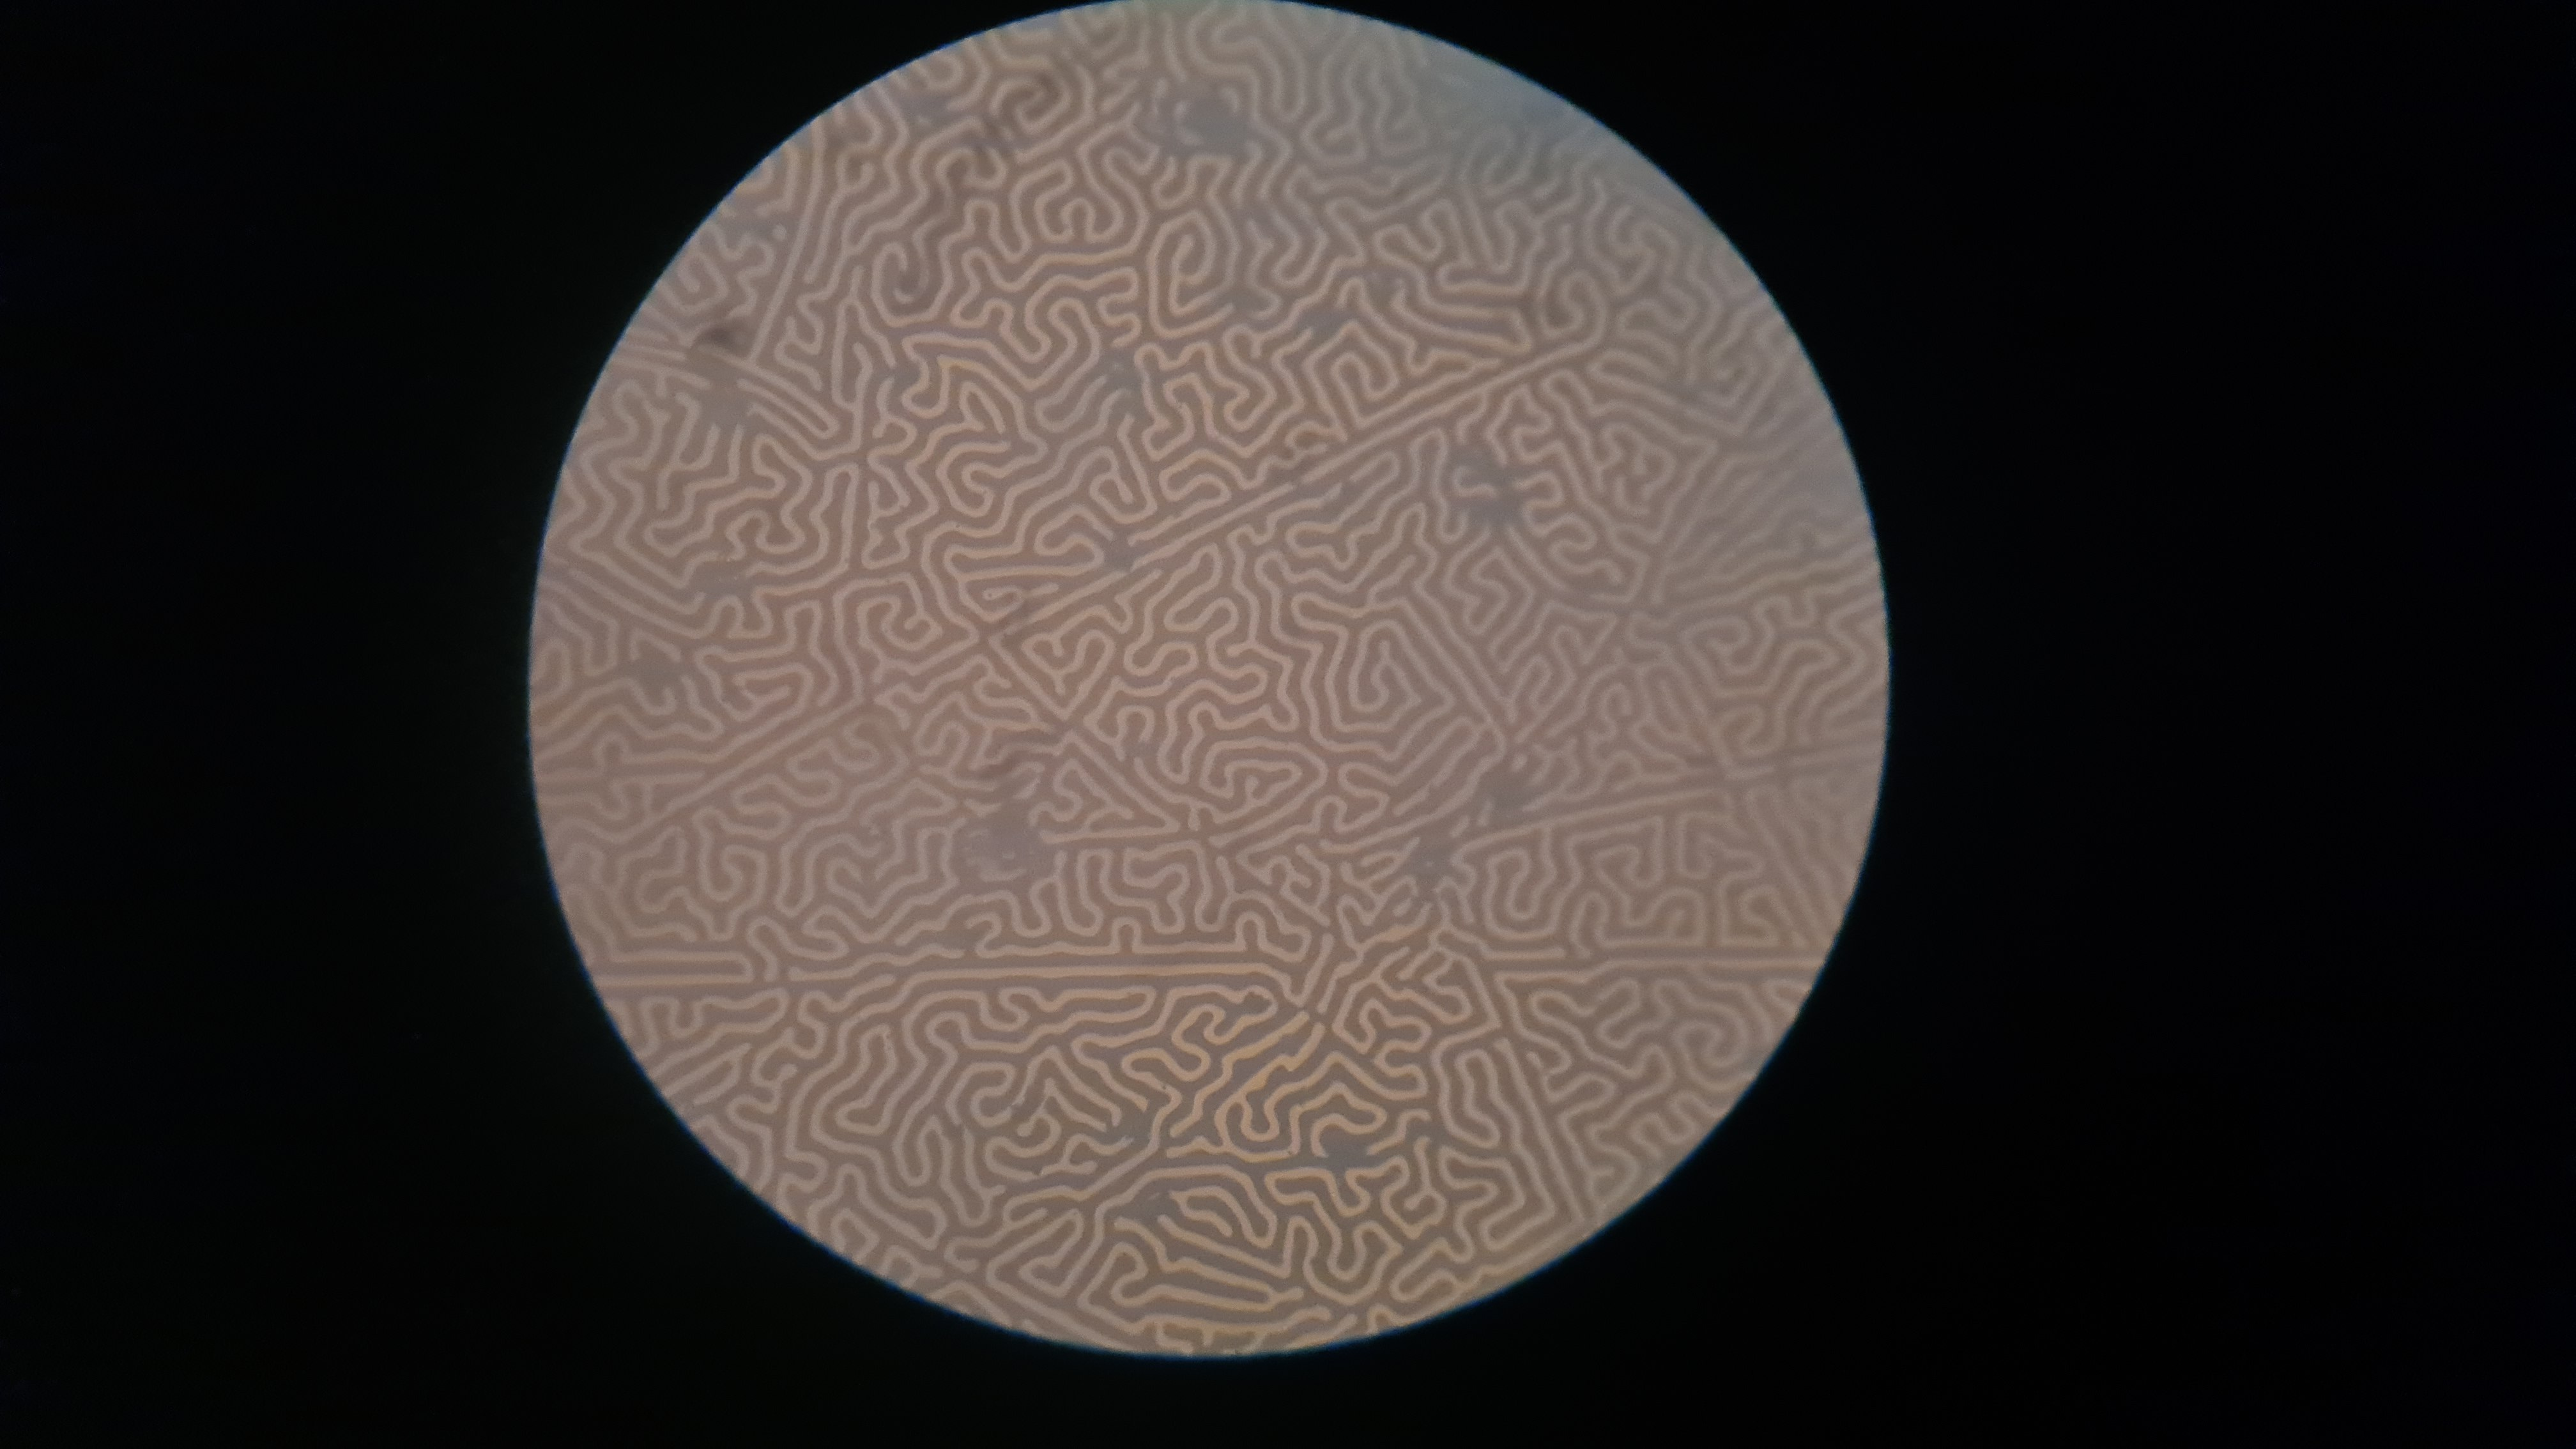
\includegraphics[width = 0.45\textwidth]{13.jpg}
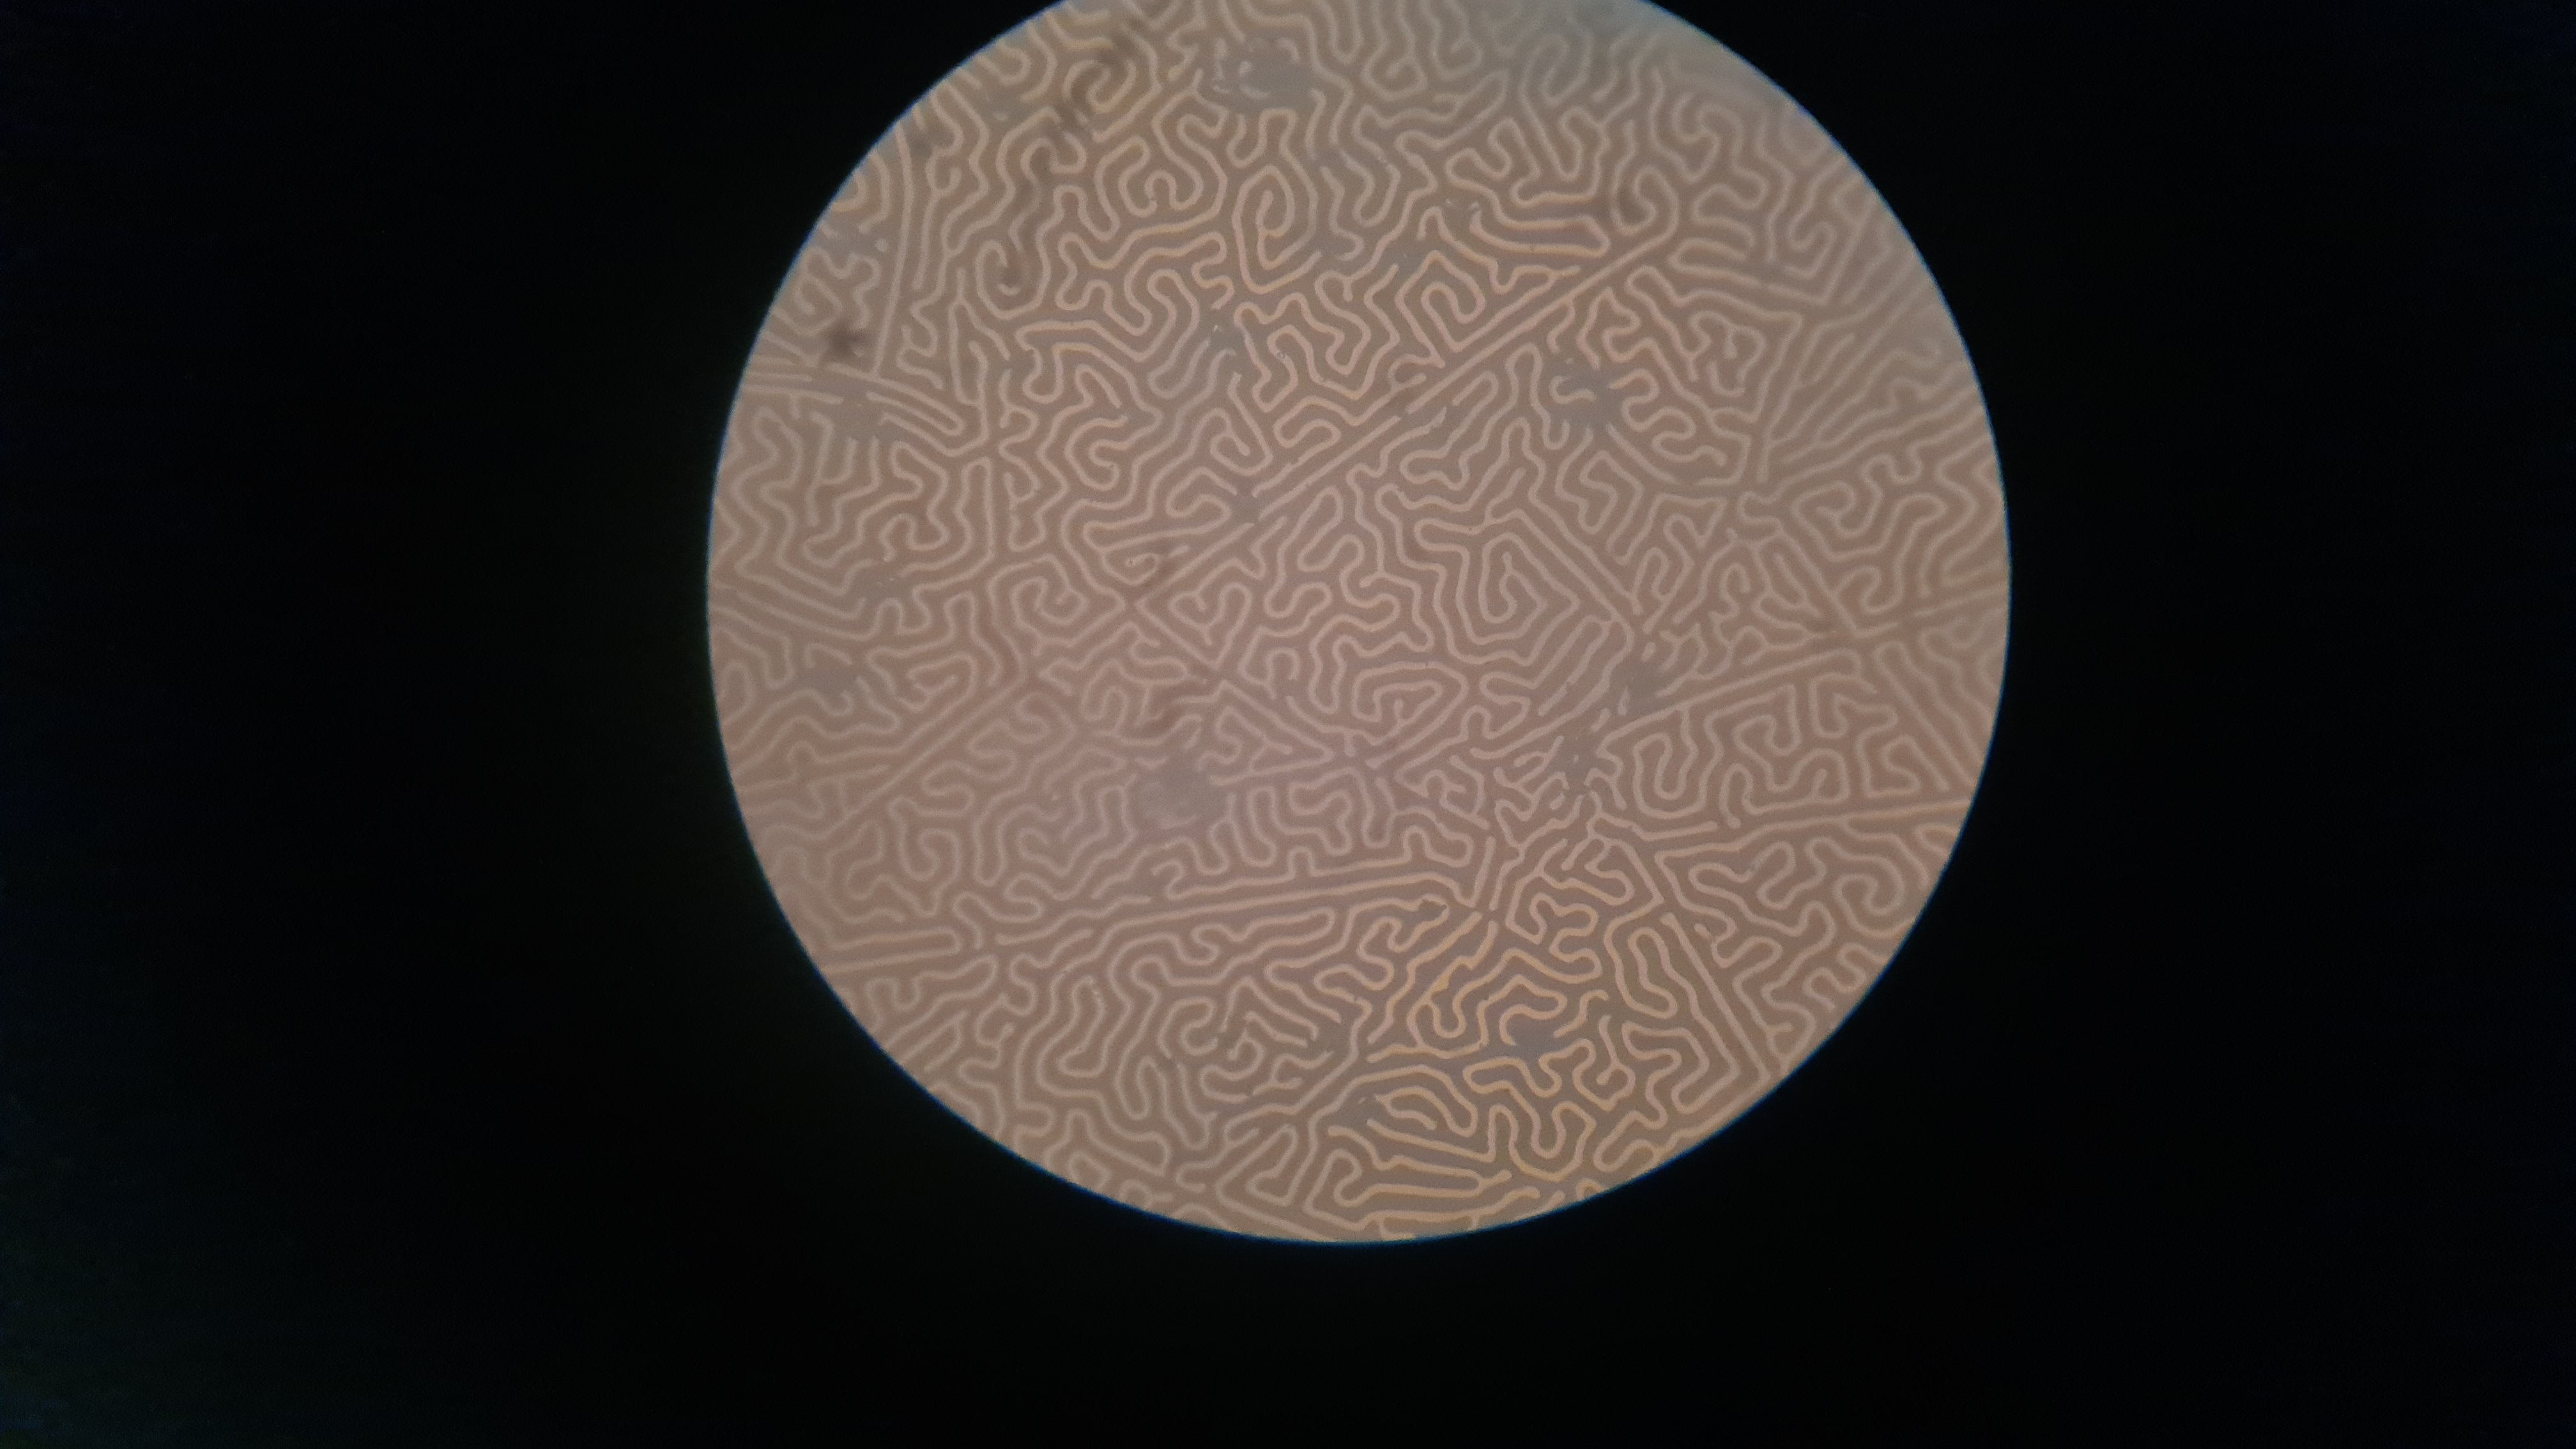
\includegraphics[width = 0.45\textwidth]{14.jpg}
\caption{Фото под номером 3 и 4 в таблице}
\end{center}
\end{figure}
\begin{figure}[h]
\begin{center}
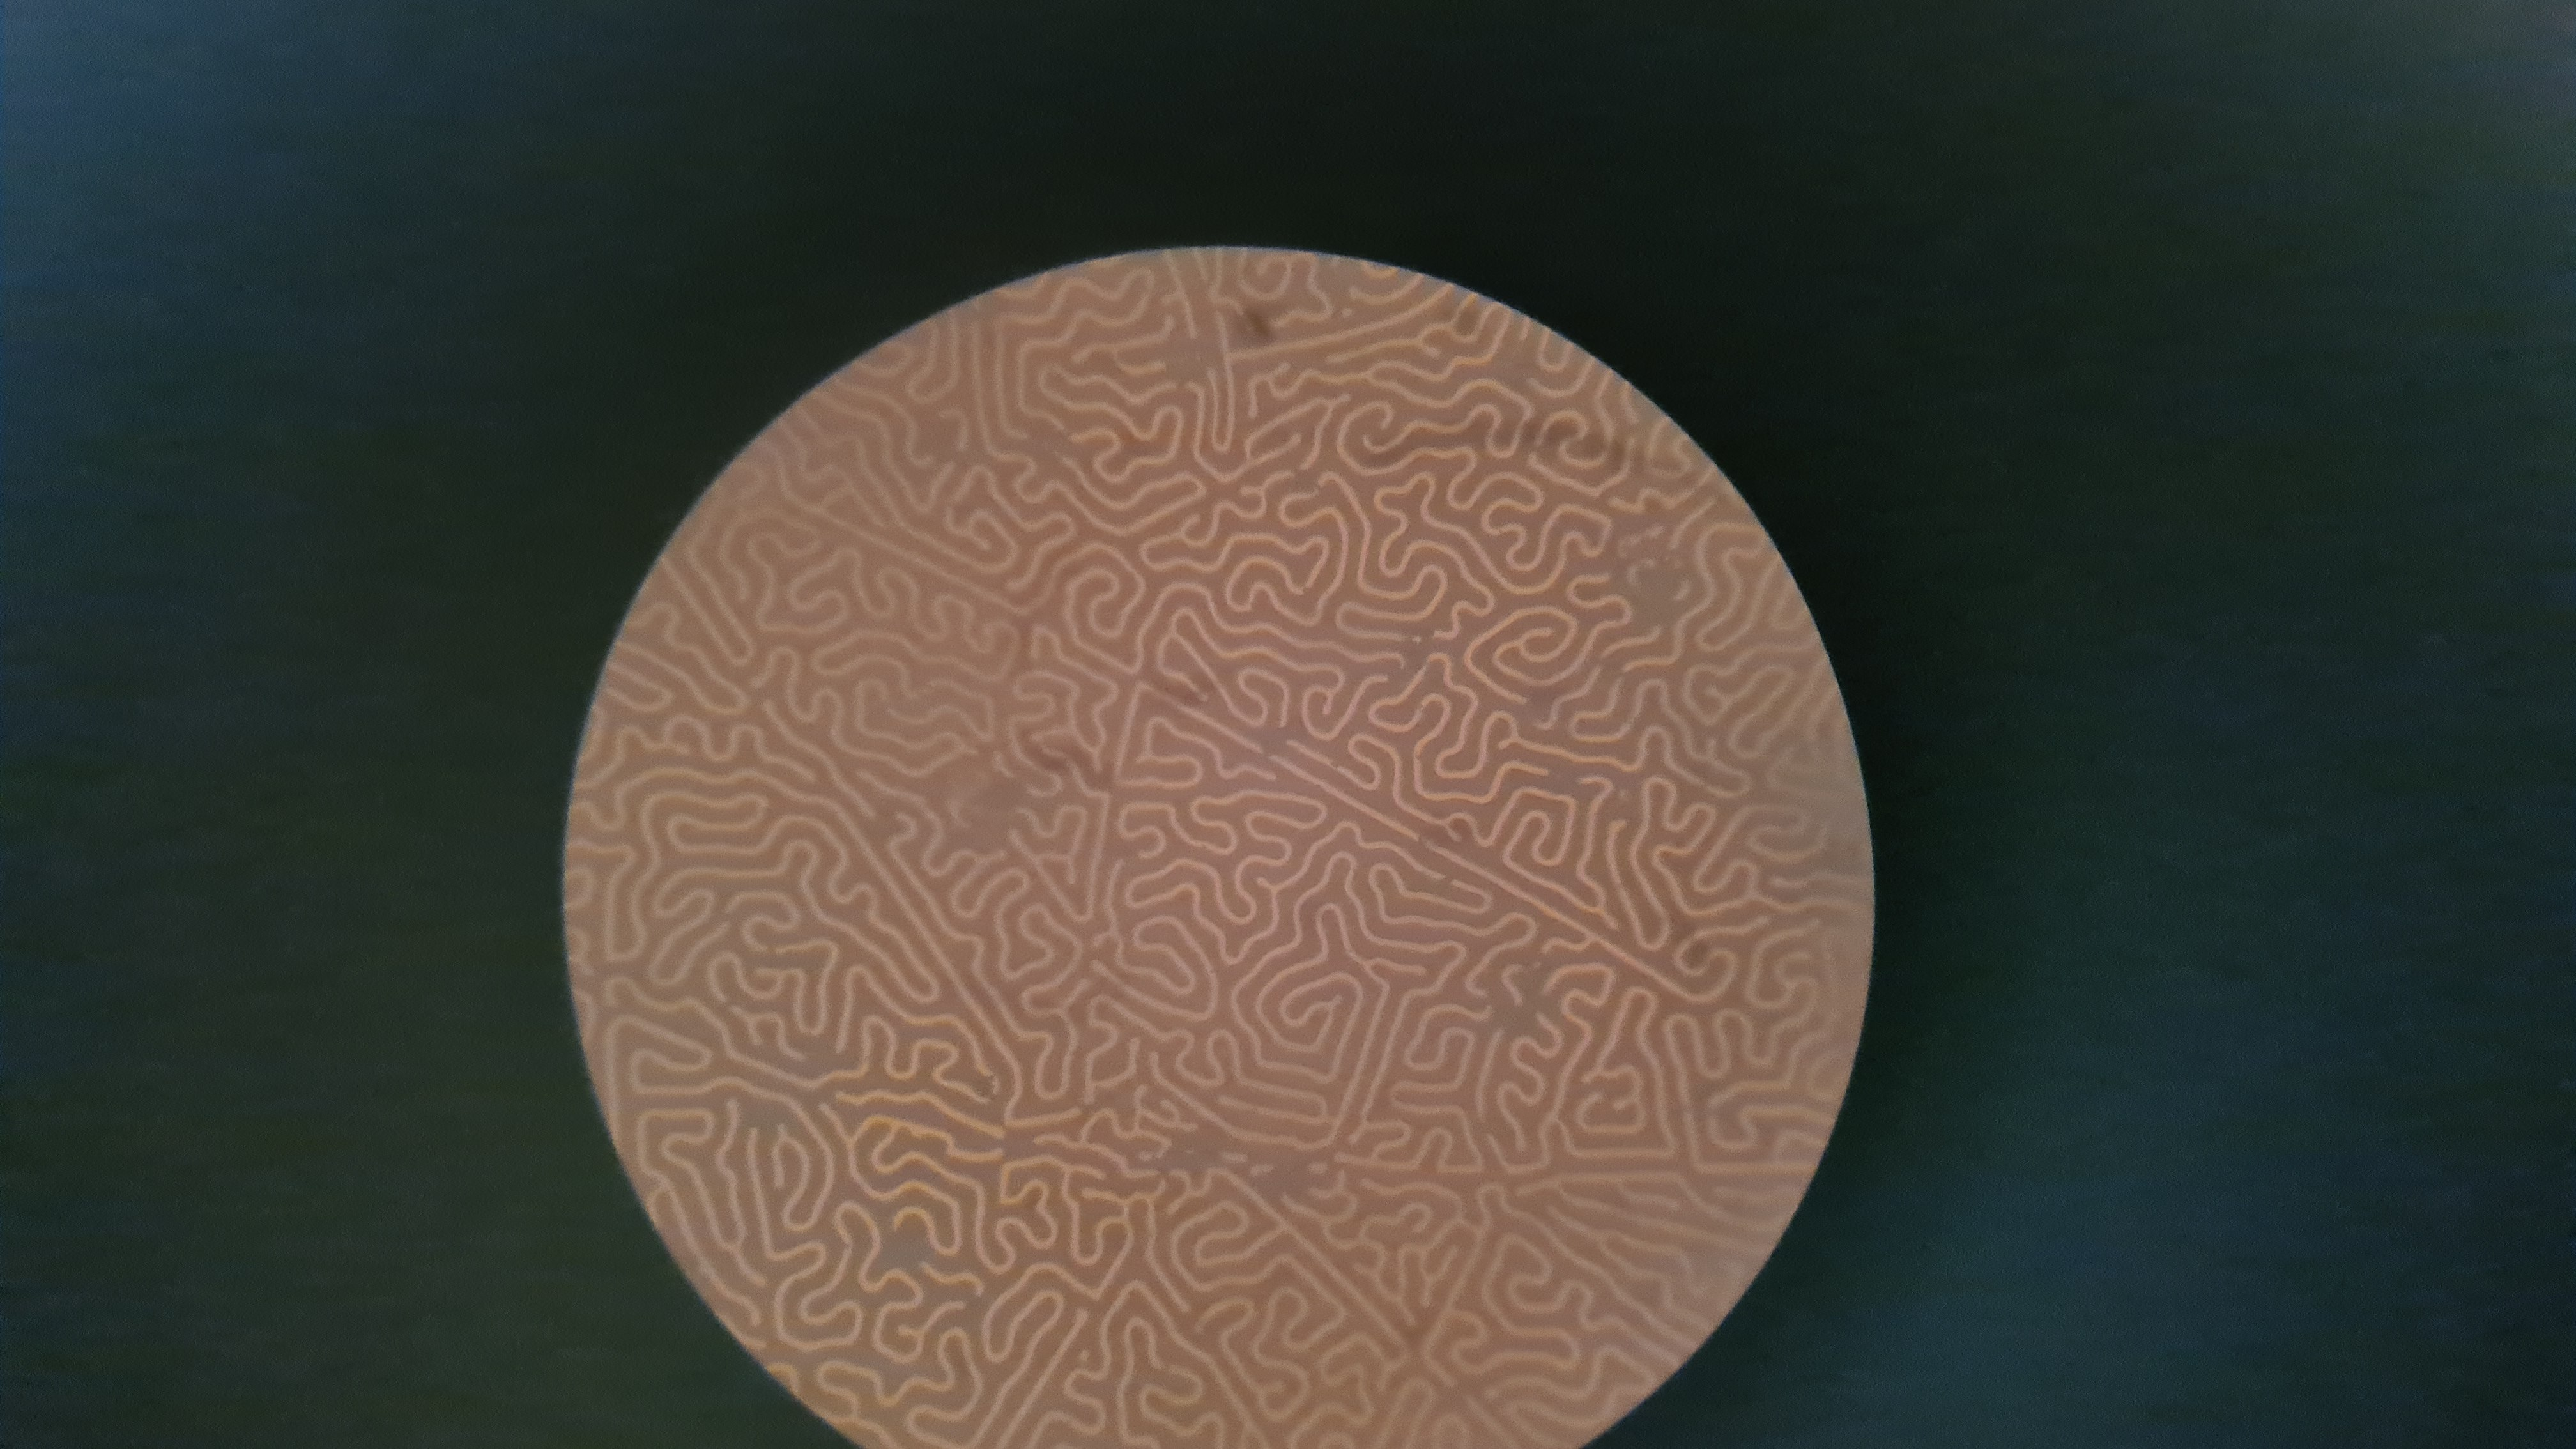
\includegraphics[width = 0.45\textwidth]{15.jpg}
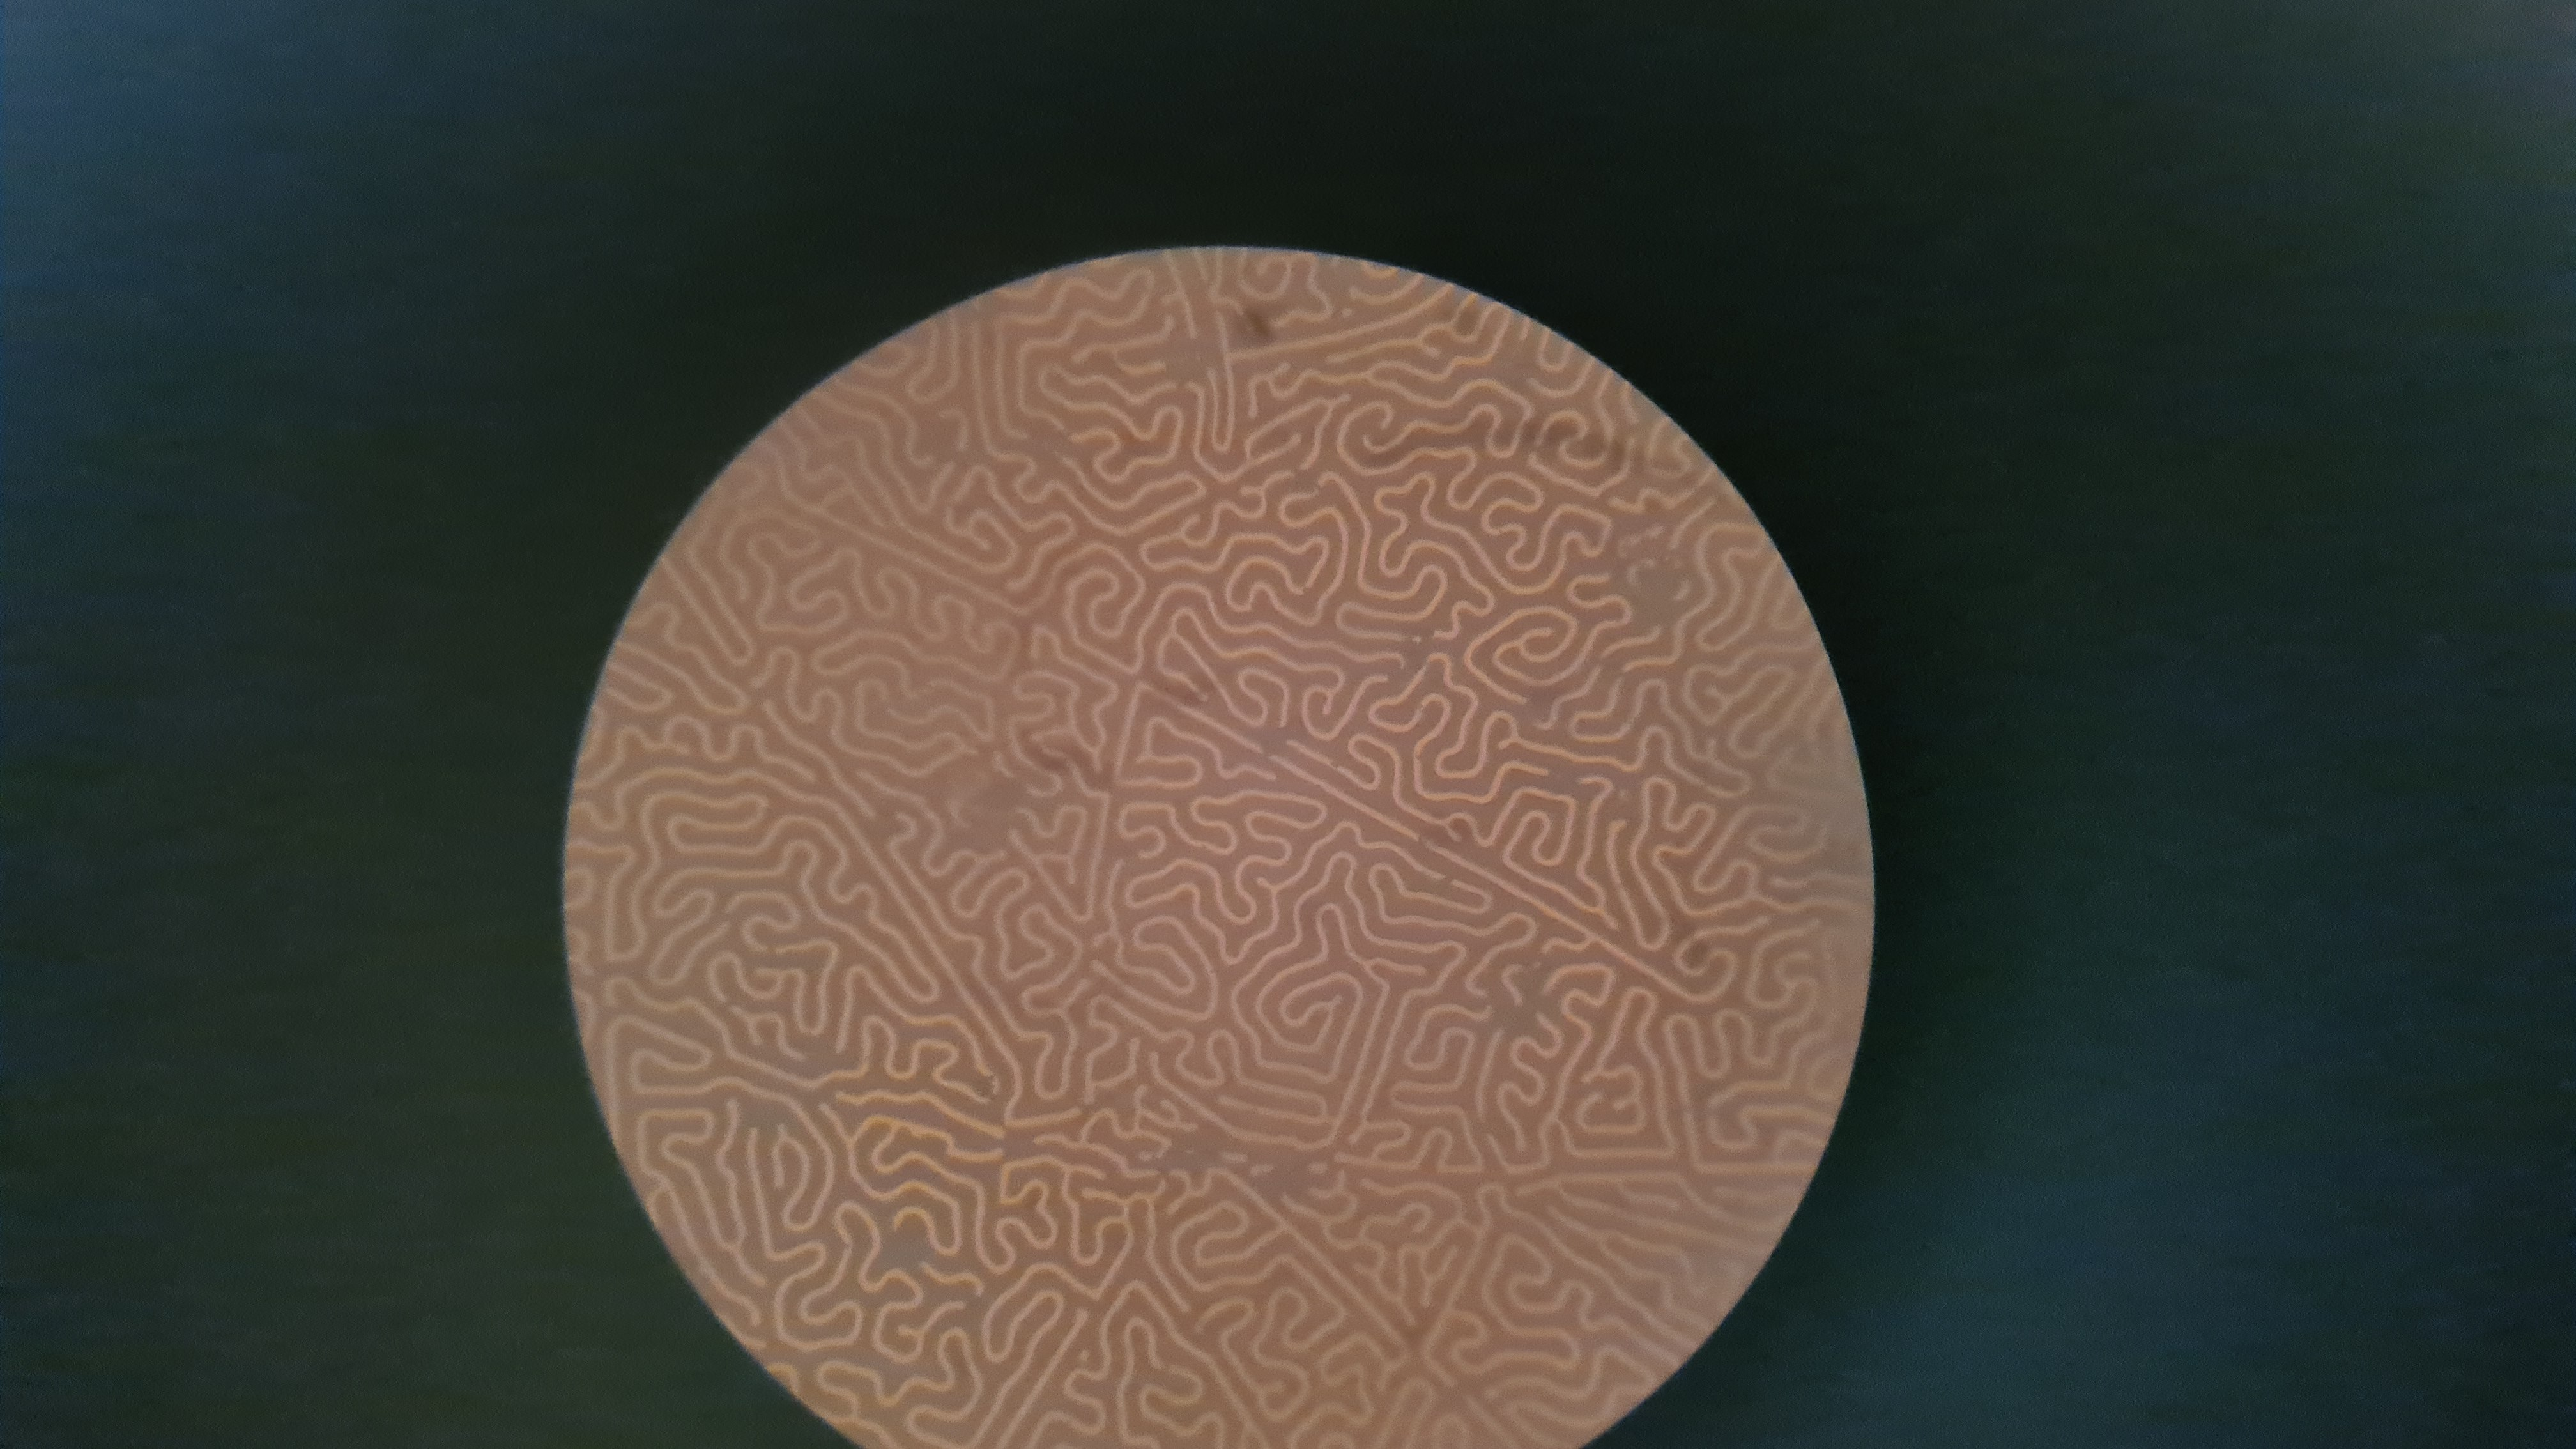
\includegraphics[width = 0.45\textwidth]{16.jpg}
\caption{Фото под номером 5 и 6 в таблице}
\end{center}
\end{figure}
\begin{figure}[h]
\begin{center}
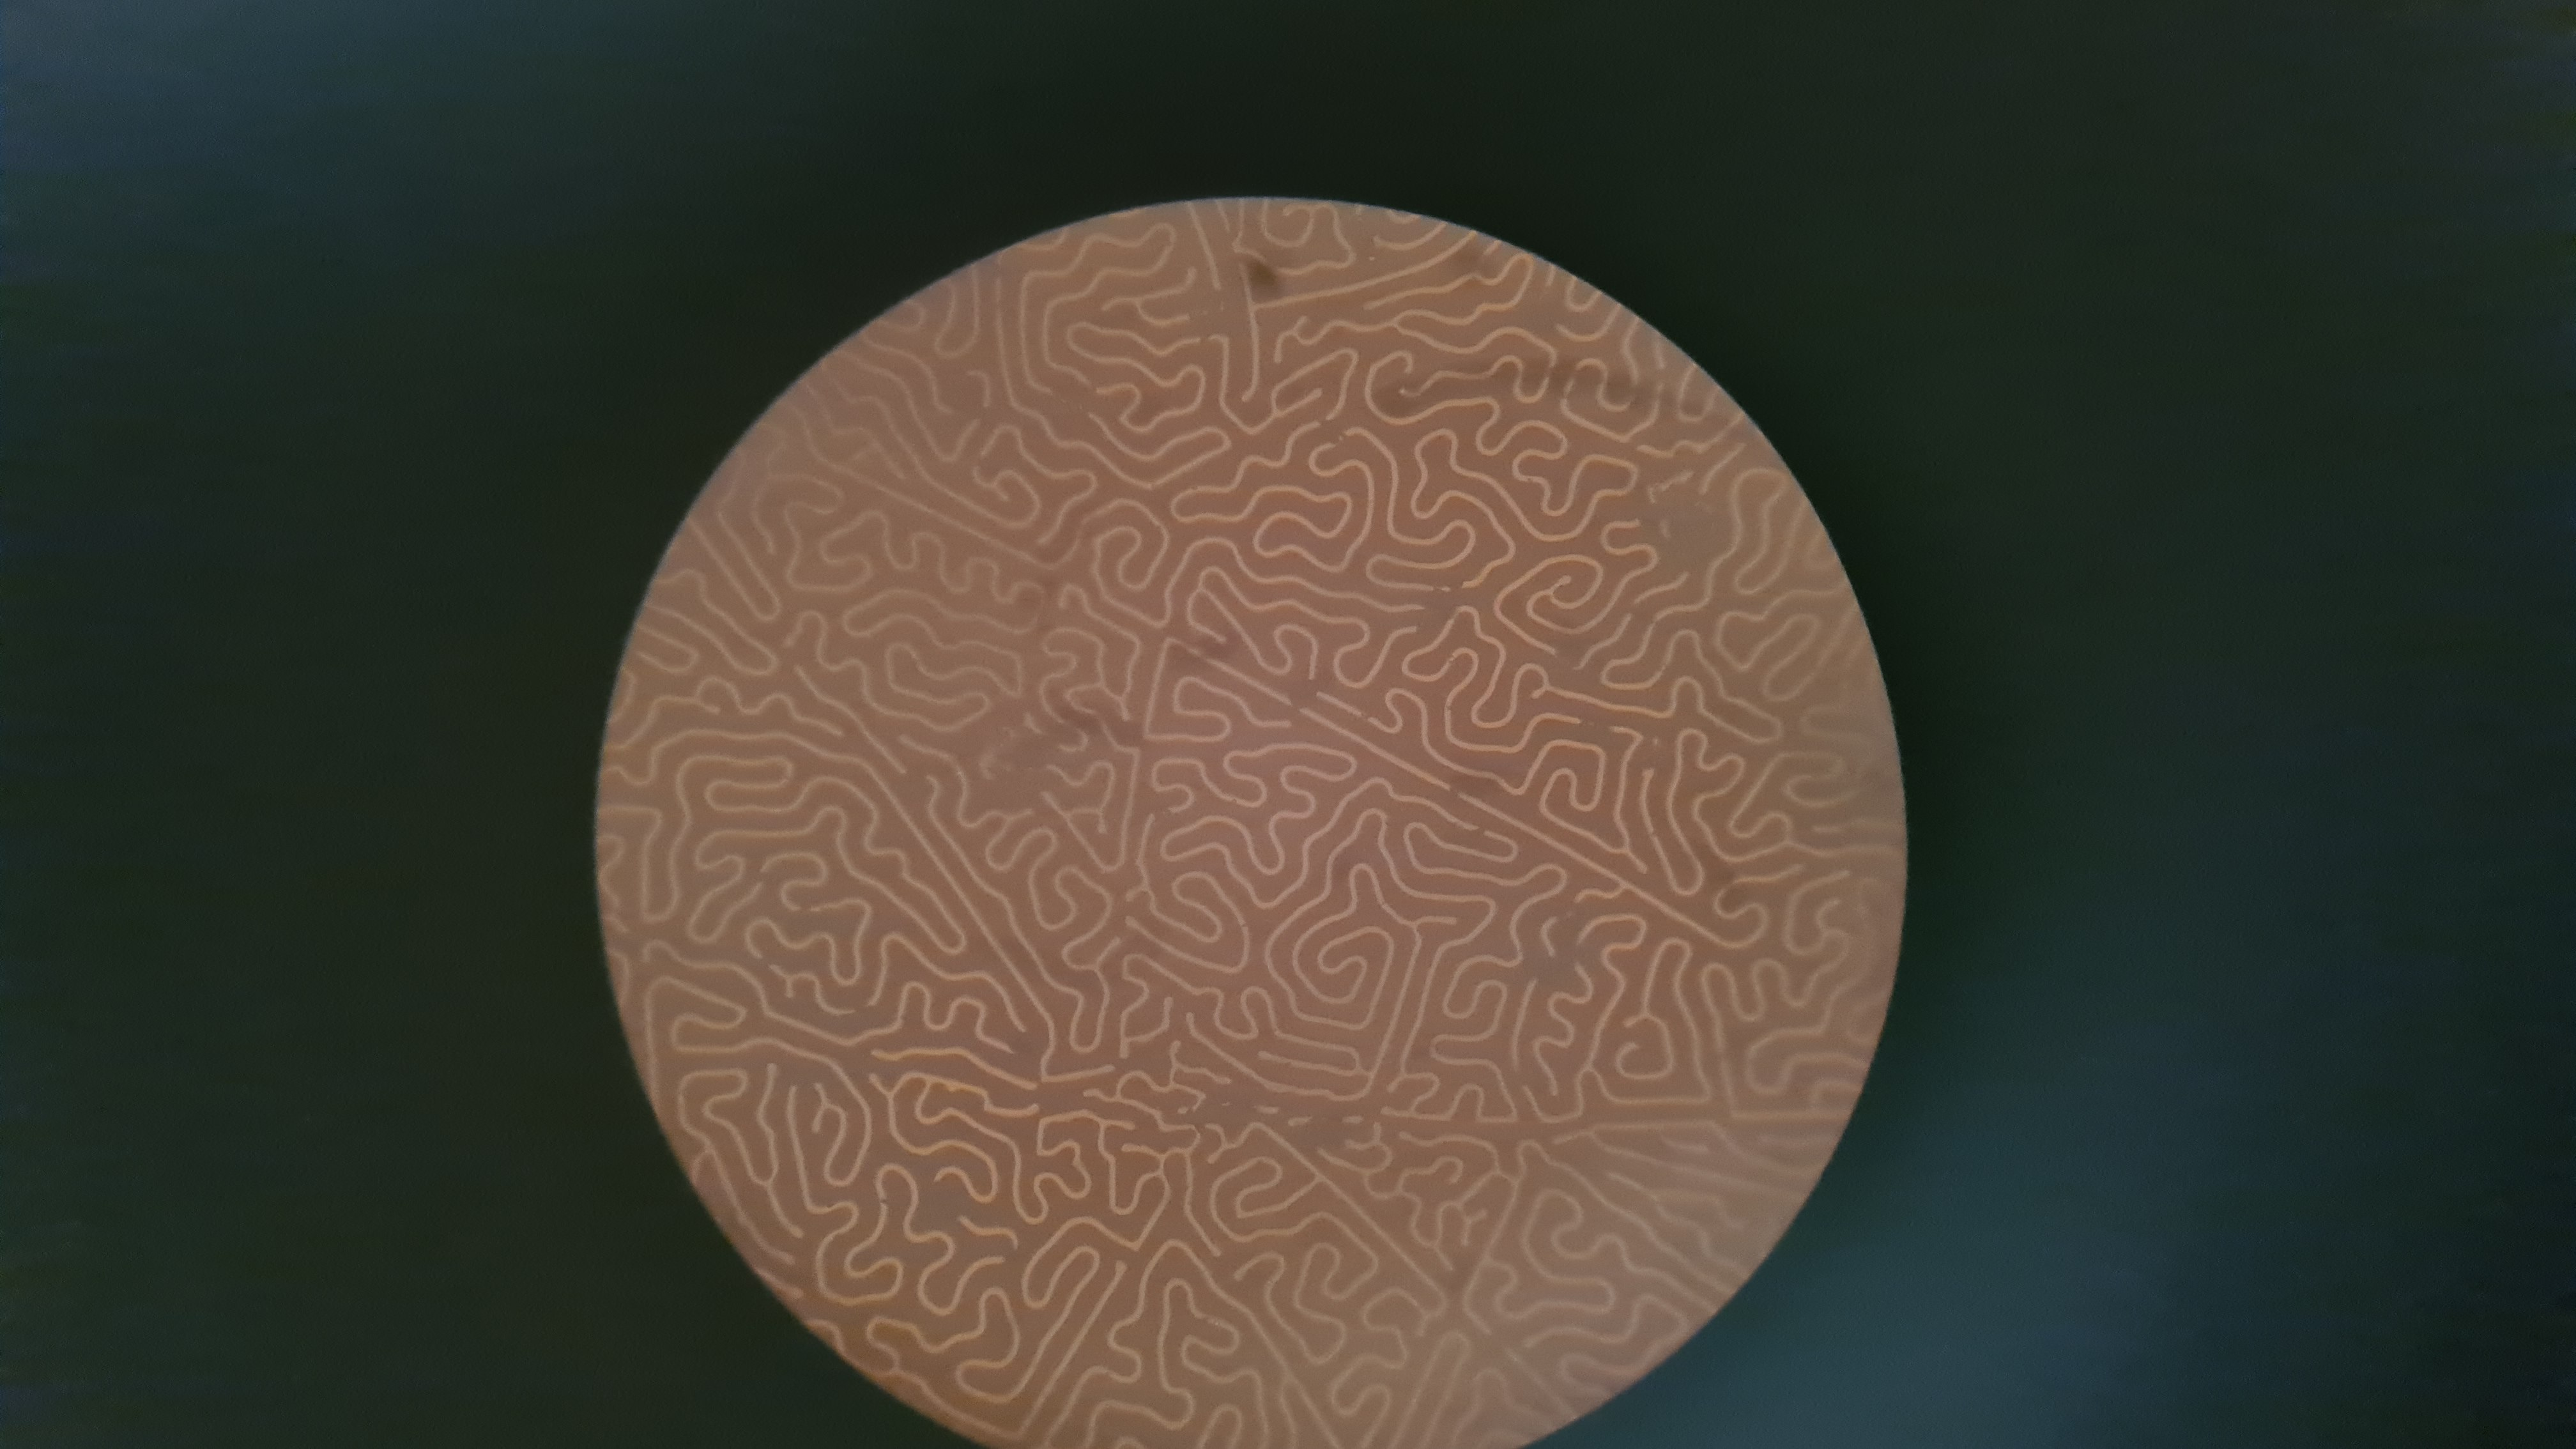
\includegraphics[width = 0.45\textwidth]{17.jpg}
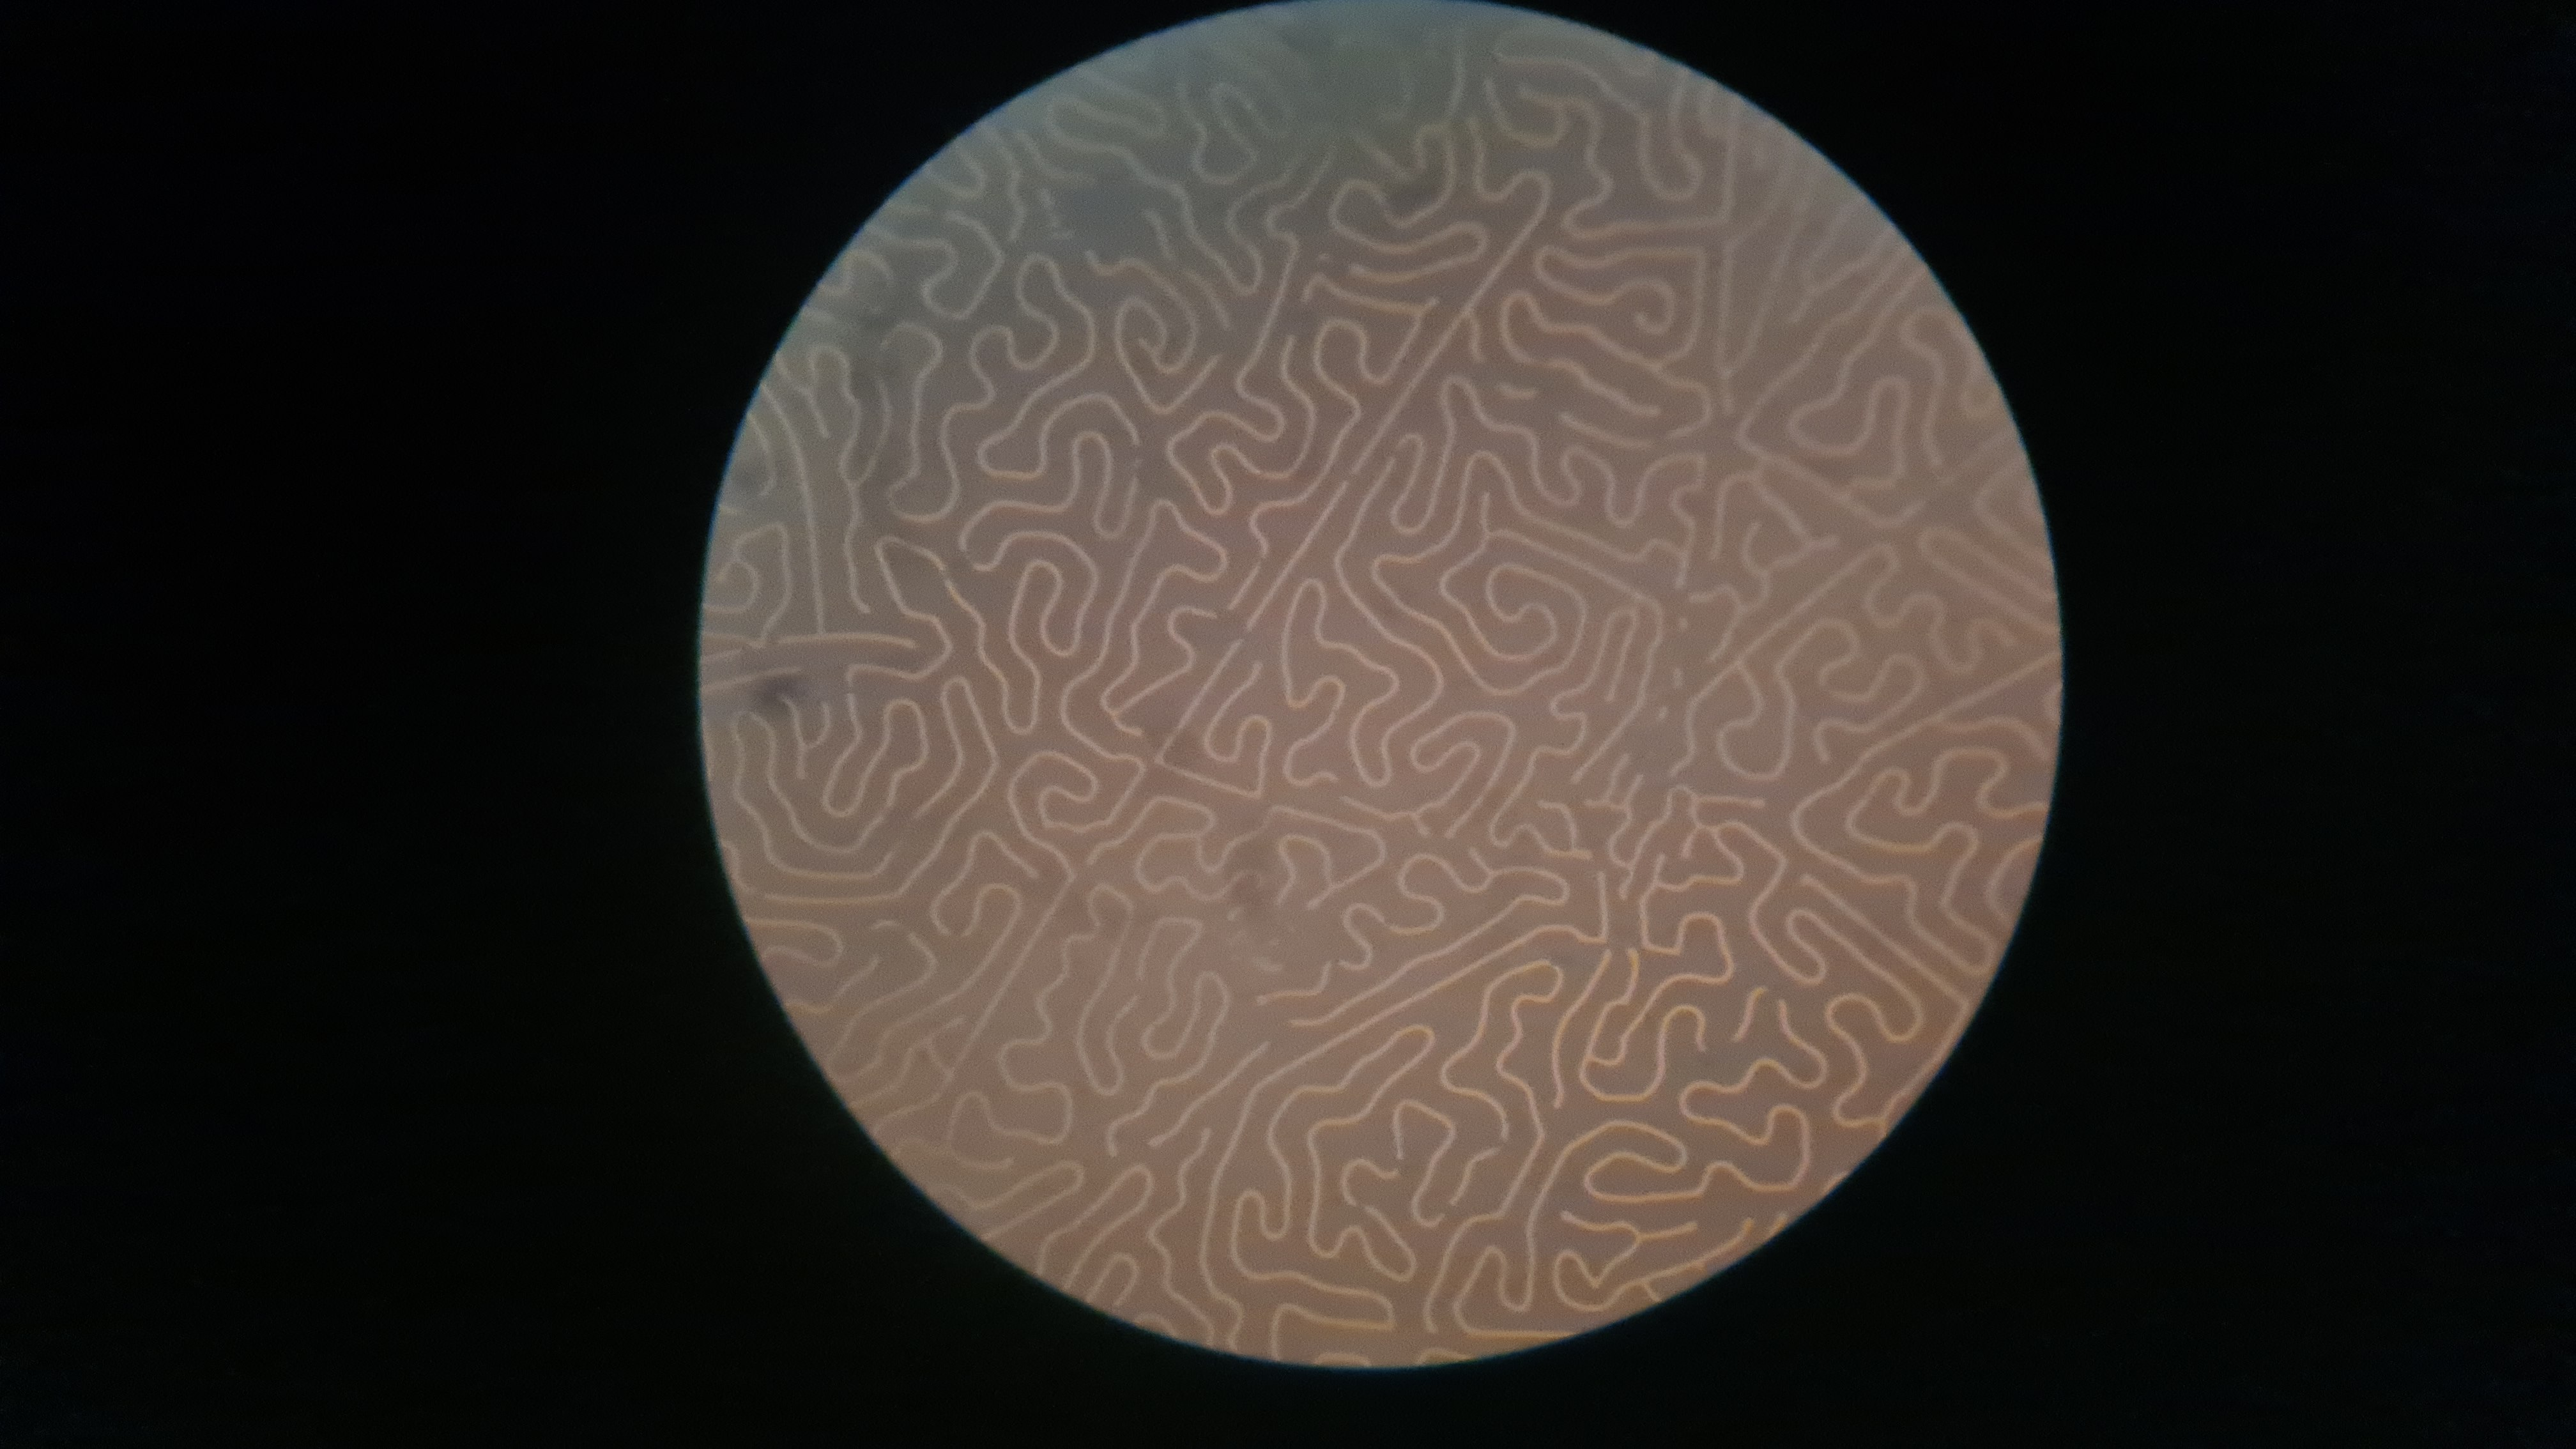
\includegraphics[width = 0.45\textwidth]{18.jpg}
\caption{Фото под номером 7 и 8 в таблице}
\end{center}
\end{figure}
\newpage
\begin{figure}[h]
\begin{center}
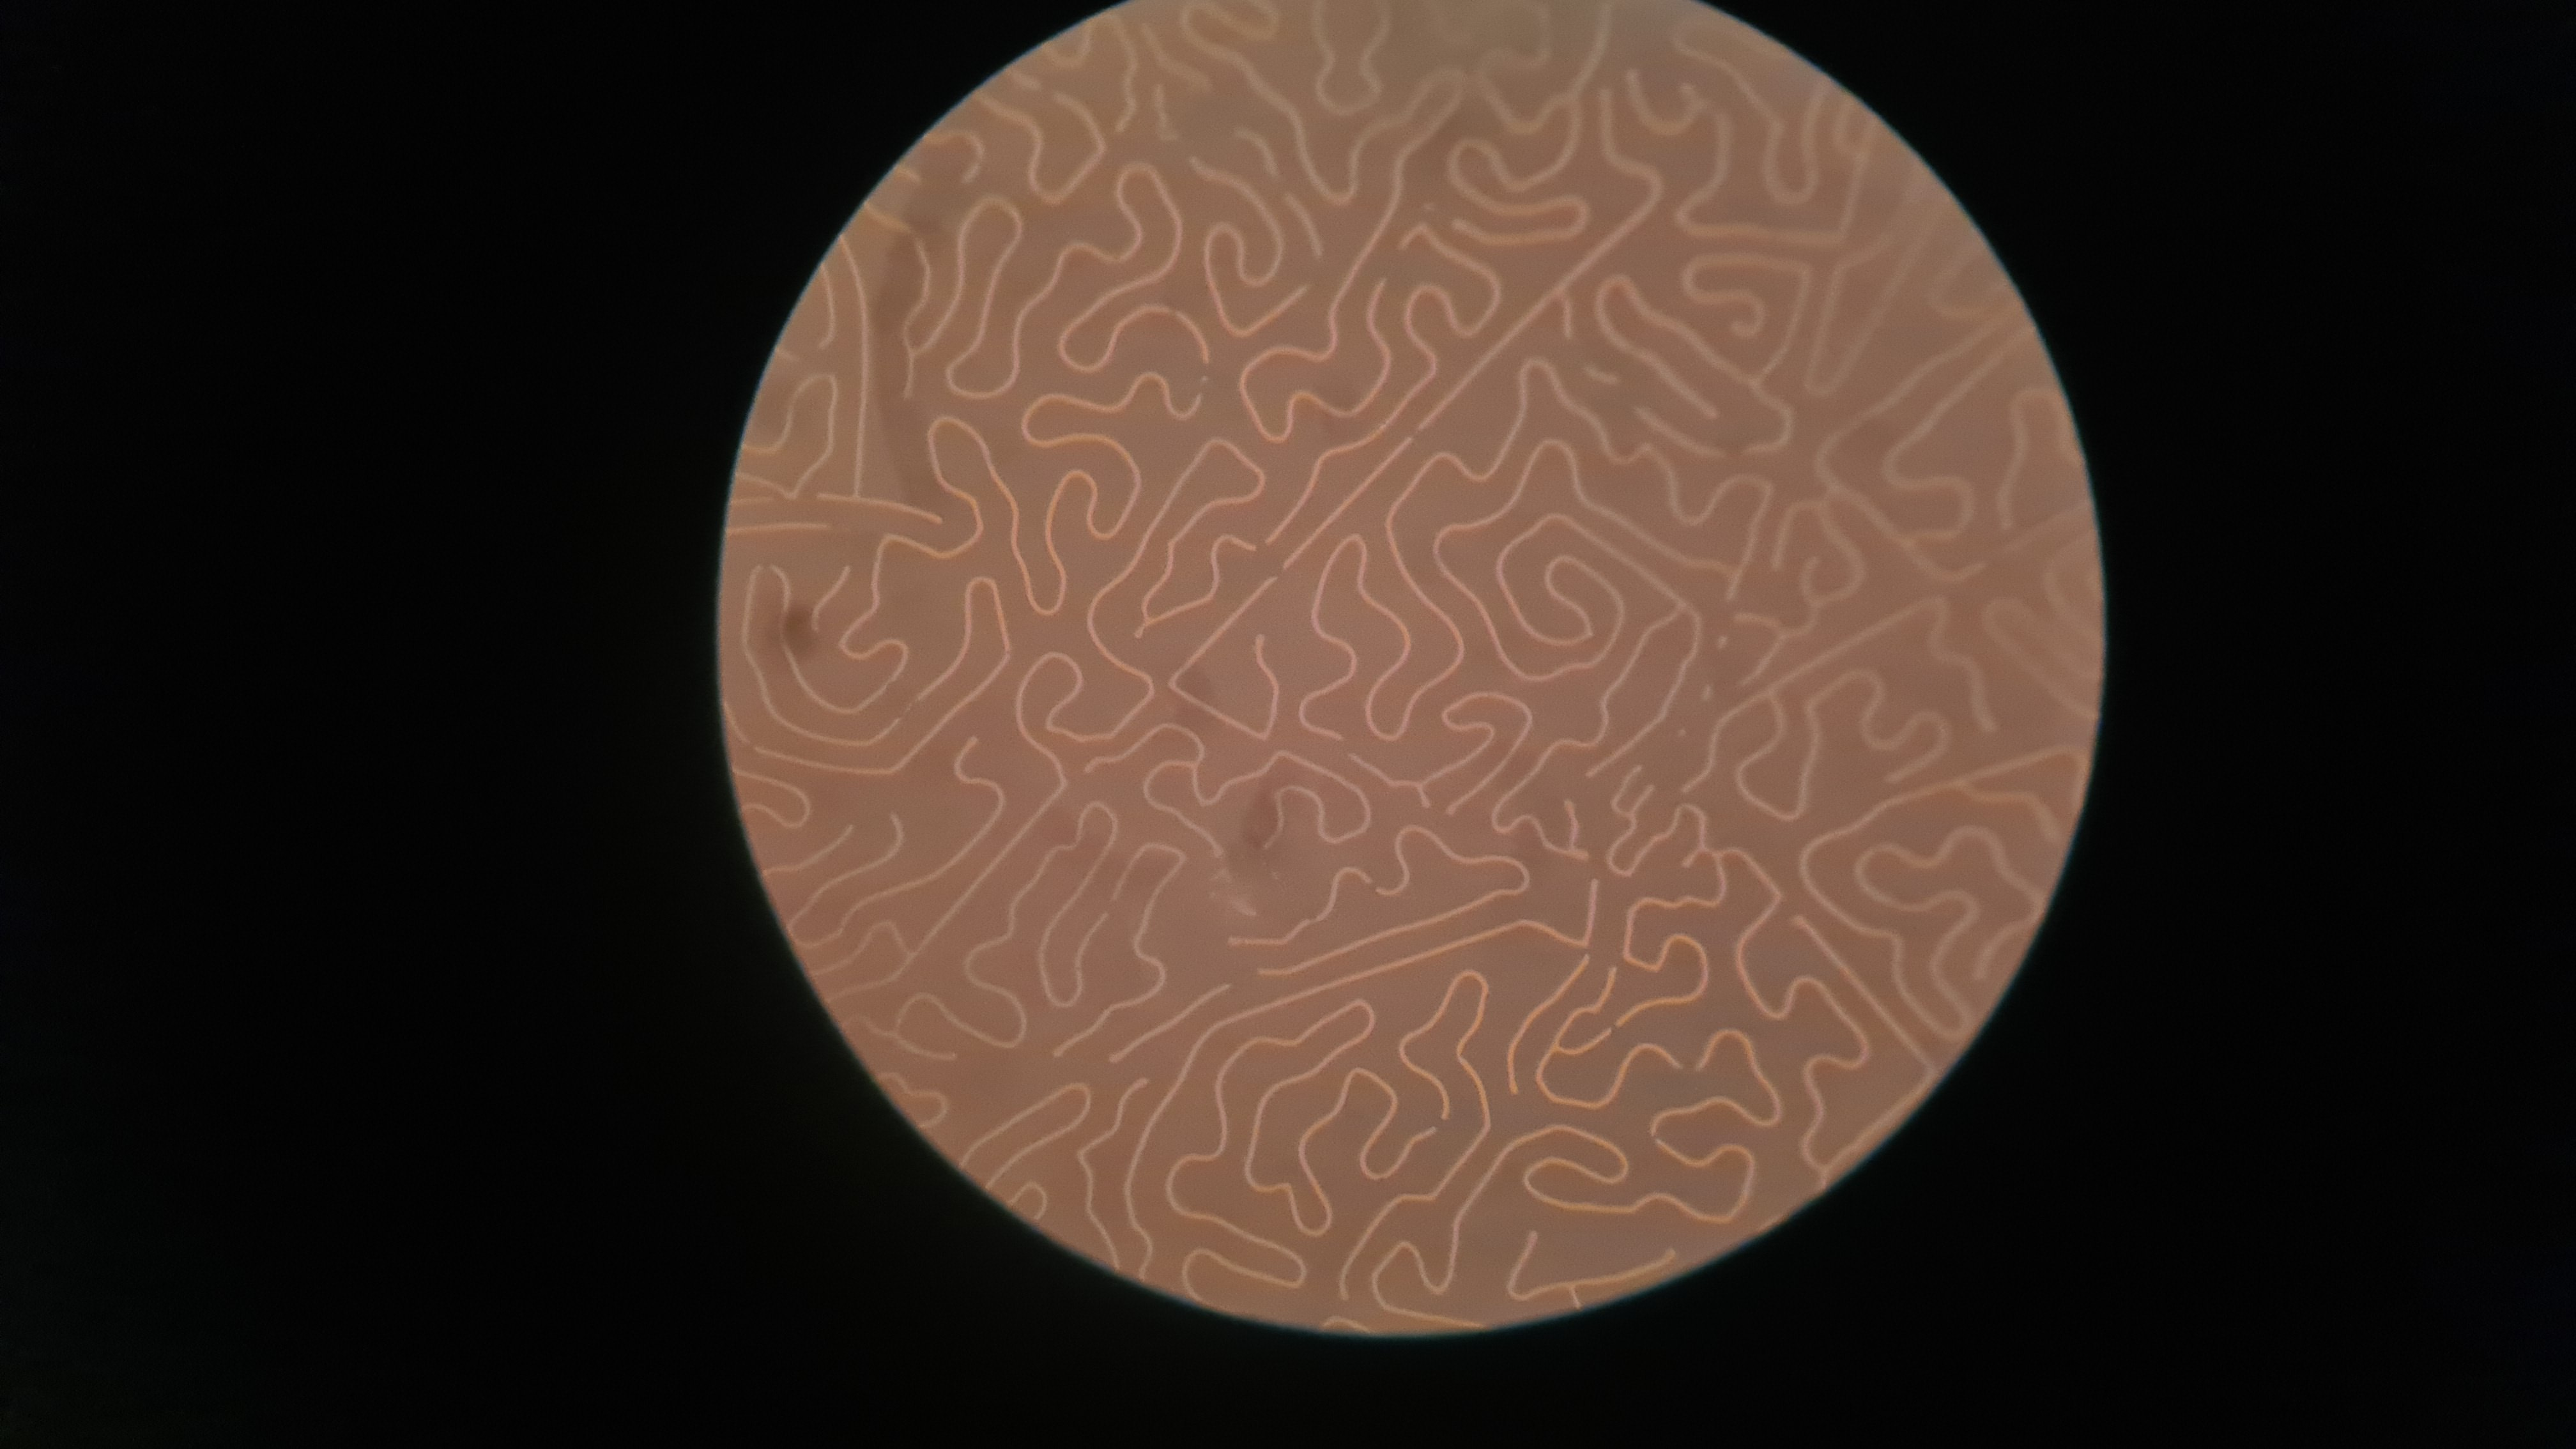
\includegraphics[width = 0.45\textwidth]{19.jpg}
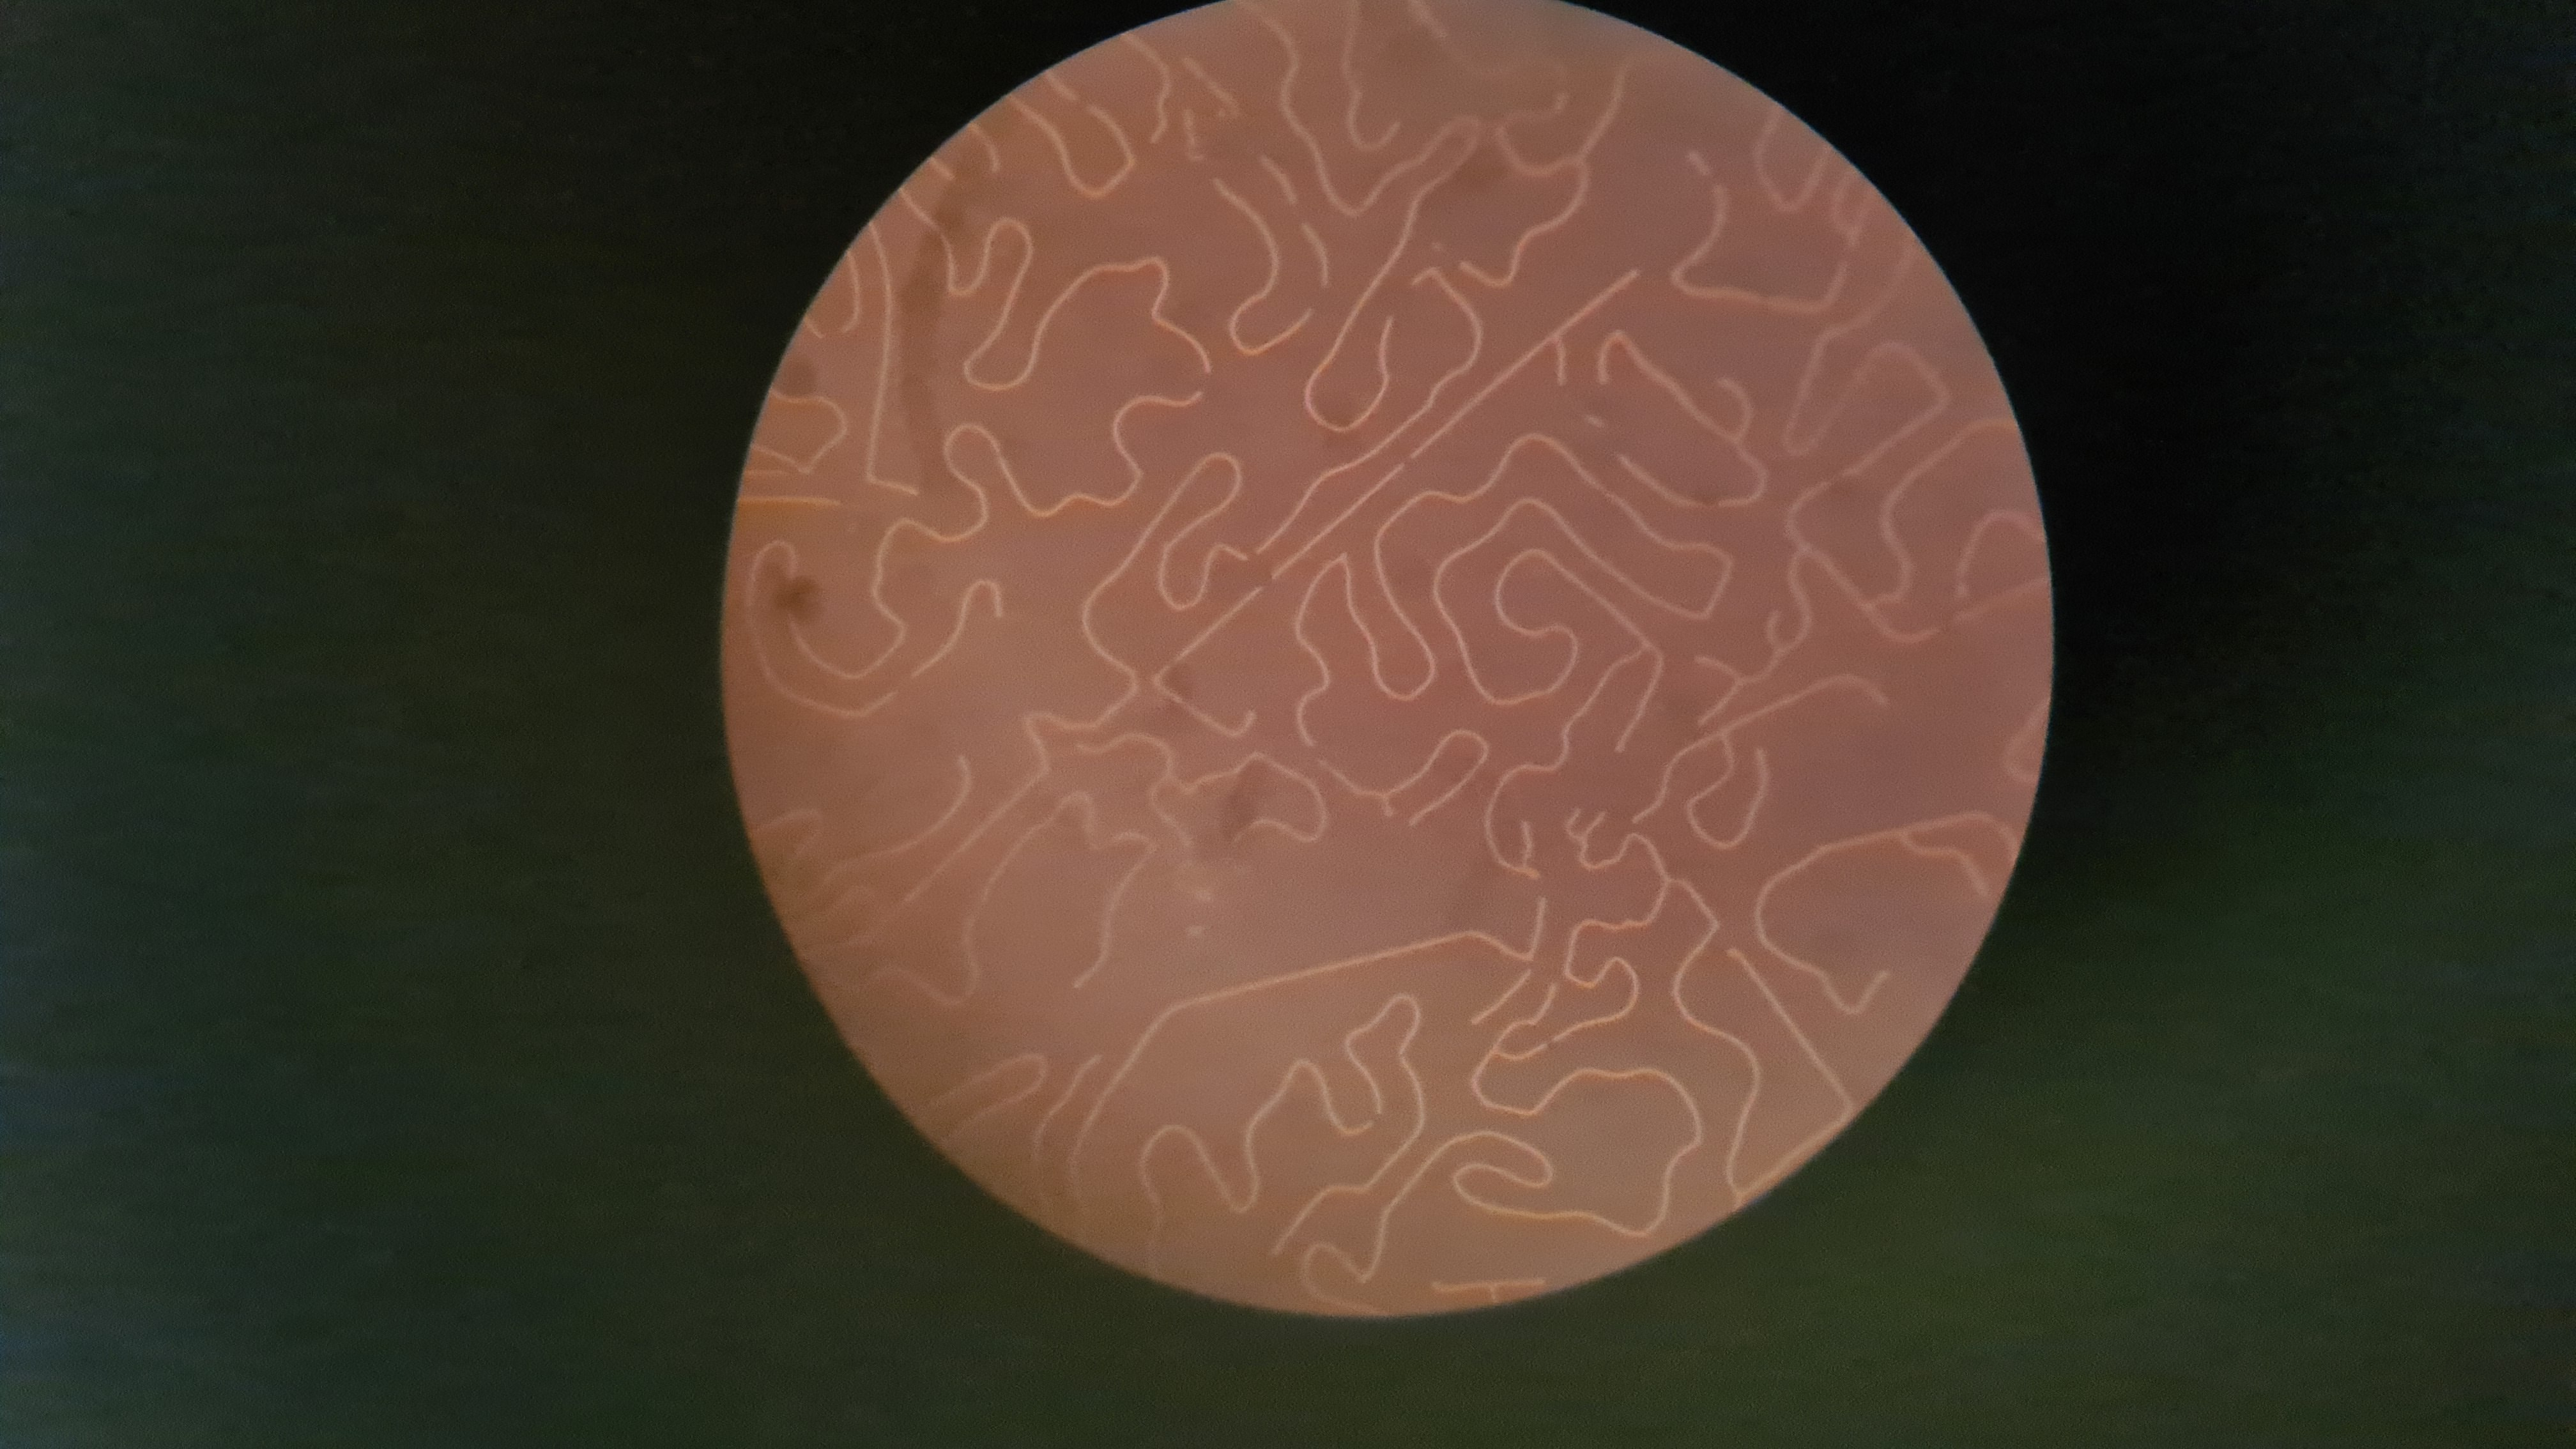
\includegraphics[width = 0.45\textwidth]{20.jpg}
\caption{Фото под номером 9 и 10 в таблице}
\end{center}
\end{figure}
\begin{figure}[h]
\begin{center}
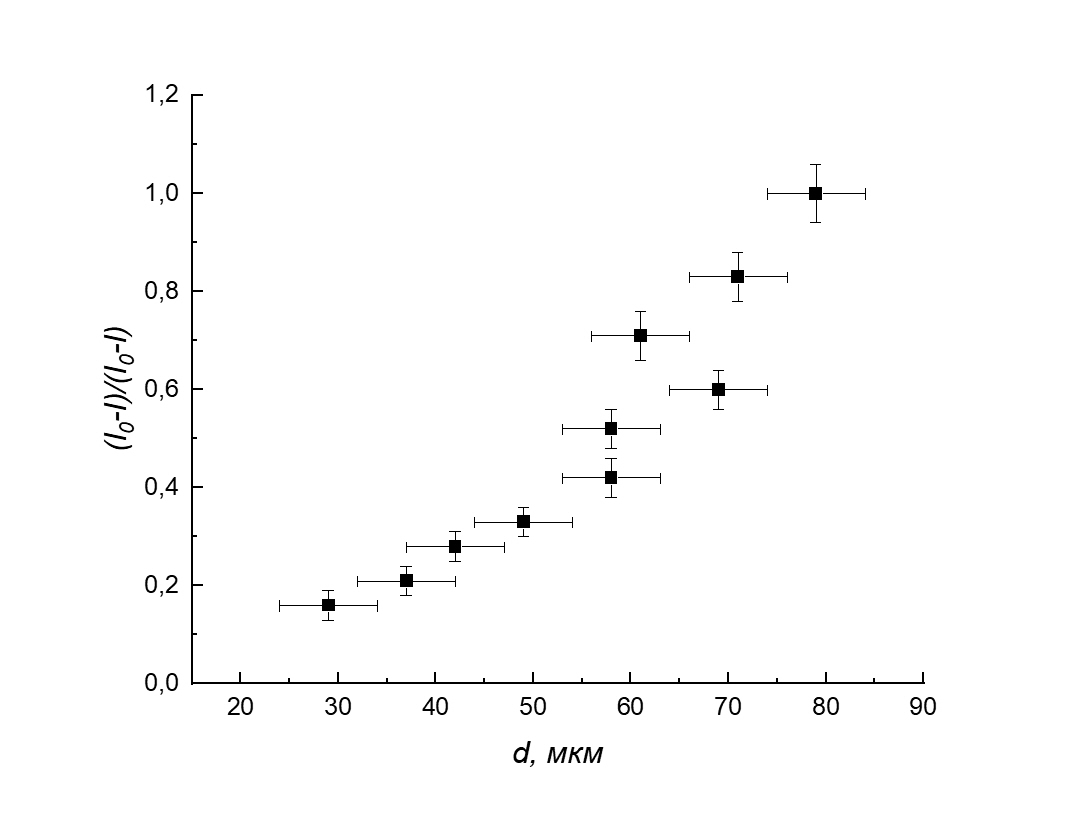
\includegraphics[width = 0.85\textwidth]{7.jpg}
\caption{Зависимость $\frac{I_0 - I}{I_0+I}$ от d}
\end{center}
\end{figure}
\section{Анализ результатов и проверка закона Кюри-Вейсса}
Полученная температура Кюри с точностью до 2 погрешностей сходится с табличным значением, равным 293,4 K. Это может быть связано с тем, что у нас неточно фиксировалась температура, из-за чего мы получали $f$ и $f_0$ для немного других температур, из-за чего увеличилась погрешность. Экспериментальная кривая при температурах больше точки Кюри выходит на прямую. Соответственно закон Кюри для парамагнитной области выполняется. Однако видно, что при высоких температурах график начинает отходить от линейной зависимости.
\section{Вывод}
В ходе данной работы мы успешно проверили закон Кюри-Вейсса для парамагнитной фазы ферромагнетика, определили Температуру Кюри гадолиния, которая сошлась с табличной и оценили значение обменного интеграла для гадолиния по теории обменного взаимодействия.
\begin{thebibliography}{3}
\bibitem{I_2}
Игошин Ф. Ф., Самарский Ю. А., Ципенюк Ю. М. Лабораторный практикум по общей физике: квантовая физика. МФТИ, 2012.
\end{thebibliography}
\end{document}
